\documentclass[letterpaper, 10 pt, conference]{ieeeconf}  

\IEEEoverridecommandlockouts
\overrideIEEEmargins

\usepackage{pgfplots}
\usepackage{xparse} 
\usepackage{amsmath} 
\usepackage{amssymb}
\usepackage{amsfonts} 
\usepackage{bbm}
\usepackage{color}
\usepackage{resizegather}
\usepackage{tikz}
\usetikzlibrary{external}
\usetikzlibrary{through}
\usetikzlibrary{plotmarks}
\usetikzlibrary{arrows,shapes}
\usetikzlibrary{plothandlers}
\usetikzlibrary{positioning}
\usetikzlibrary{calc}
\usepackage{float}
\usepackage[hyphens]{url}



\usepackage{graphicx}
\usepackage{epstopdf}
\usepackage{caption}
\usepackage{subcaption}

\usepackage{hyperref}
\usepackage{cleveref}
\usepackage{multirow}

% for biblatex and mklatex
%\usepackage[backend=bibtex,style=ieee,natbib=true]{biblatex} %added
%\addbibresource{ieeeabrv.bib} % Abbreviations
%\addbibresource{ref.bib} %added
\bibliographystyle{IEEEtran}
%\usepackage{nomencl} 
%\makenomenclature

%mycal below
\graphicspath{{images/}}
\DeclareMathOperator*{\argmax}{\arg\max} %added by Mycal
\usepackage{adjustbox} %added by mycal
\usepackage{amsmath}
\usepackage{algorithm}
\usepackage[noend]{algpseudocode}

\title{DCG-UPUP-Away: Automatic Symbol Learning through Grounding to Unknowns}
\author{Mycal Tucker, Derya Aksaray, Rohan Paul, and Nicholas Roy% <-this % stops a space
\thanks{All authors are with the Computer Science and Artificial Intelligence Laboratory (CSAIL),
Massachusetts Institute of Technology, Cambridge, MA 02139, USA
{\tt\small \{mycal,daksaray,rohanp,nickroy\}@csail.mit.edu}}%
\thanks{It appears as if acknowledgments sometimes go here, but there's also the acknowledgment section at the end. What's the difference?}% <-this % stops a space
}

\begin{document}
\maketitle
\thispagestyle{empty}
\pagestyle{empty}

\begin{abstract}
This work addresses the symbol grounding problem, that is, understanding the ``meaning" of natural language within a robot's workspace. The state of the art models used in the grounding problem typically assume a fixed set of phrases or objects that are defined a priori to mission. However, the real world is full of unexpected objects that are nearly impossible to anticipate and therefore train for. This paper proposes a model called the ``Distributed Correspondence Graph - Unknown Phrase, Unknown Percept - Away" that explicitly represents unknown phrases and objects as unknown symbols and enables to reason about objects outside the field of view. Moreover, the model is capable of acquiring new symbols in an online fashion. The effectiveness of the model is evaluated via simulations and real experiments in terms of grounding and learning new phrases and objects.

%Research in automatic natural language grounding, the problem of robots associating phrases with realworld objects and actions, offers a tantalizing reality in which untrained humans can operate sophisticated robots. 

%Current techniques for training robots to understand natural language, however, assume that there is a fixed set of phrases or objects that the robot will encounter during deployment. 

%Instead, the real world is full of confusing jargon and unique objects that are nearly impossible to anticipate and therefore train for. 
%This paper presents a model called the Distributed Correspondence Graph - Unknown Phrase, Unknown Percept - Away (DCGUPUP- Away) that augments a previously successful model by explicitly representing unknown phrases and objects as unknown, as well as reasoning about objects that are not currently perceived. 
%Furthermore, experimental results in simulation,
%as well as a trial run on a physical turtlebot, validate the
%effectiveness of DCG-UPUP-Away in grounding and learning
%new phrases.
\end{abstract}

\printnomenclature %I have no idea what this does

\section{Introduction}
Recently, there has been a great interest in human-robot teaming in civilian (e.g., at factories, hotels, hospitals, homes) and military (e.g., reconnaissance) applications. Communication plays an important role in effective teaming between humans and robots. One way of communication is via natural language, which provides a rich, intuitive, and flexible medium. Accordingly, the grounding problem in the literature addresses the question of how a robot can understand the meaning of a natural language command in the context of its world model (e.g., \cite{g3,dcg,adcg2016}). 
%However, this requires a robot to understand natural language commands  domains including, but not limited to, Robots must be able to understand natural language if they are to efficiently collaborate with humans. In order to achieve this goal, the problem of associating phrase with real-world objects and actions, commonly referred to as the grounding problem, has emerged as a focus of new research in robotics (\textcolor{blue}{REF: G3,DCG, etc.}).

The existing methods to solve the grounding problem make two primary assumptions. First, they assume a fixed set of phrases that can constitute the commands and a fixed set of objects that exist in the world model. Thus, such methods typically fail to reason about unknown phrases or objects that have never been encountered (e.g., in the training process).
Second, these methods often assume that the location of the object being grounded to is known (e.g., the phrases refer to the objects that are currently perceived or localized within a known map).
As a result, a robot using these methods tends to pick the most likely perceived grounding rather than exploring its surroundings.

Note that such assumptions do not typically reflect the reality. For example, humans tend to use context-specific lexicons in their daily life, or they often refer to objects whose locations may be unknown. To deal with such cases, training a robot to know the meaning of every possible word is infeasible and inefficient. Also, attempting to reason over the space of all possible maps is similarly computationally infeasible.

\begin{figure}[t!]
	\centering
	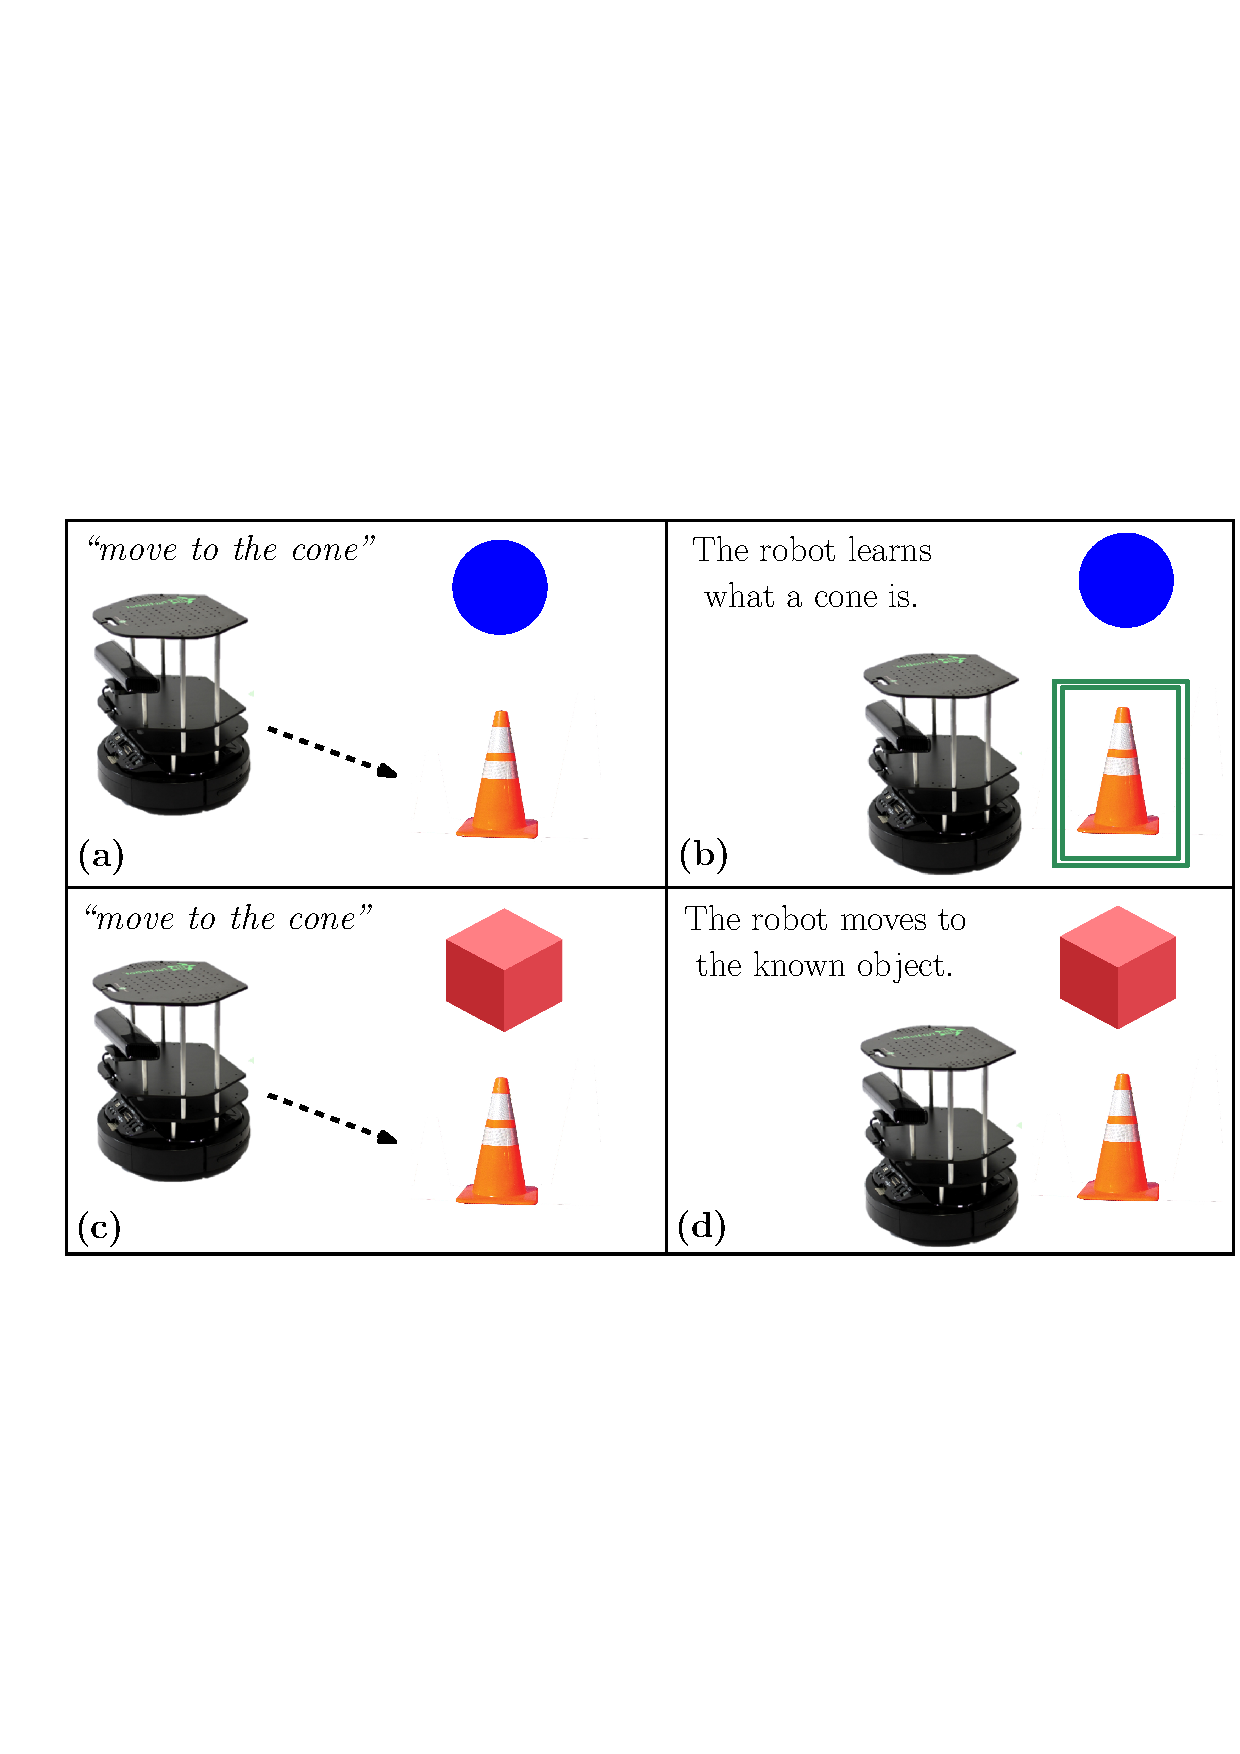
\includegraphics[width=\columnwidth]{motivation.pdf}
	\caption{An illustration of learning and grounding an unknown object. The robot (a) knows what a sphere is, (b) learns what a cone is, (c) sees a cone again, (d) moves towards the cone that is a known object from now on.} %the proposed model DCG-UPUP-Away, which has been trained only with cubes, spheres, and cylinders; and it may ground phrases to known perceived objects (1), unknown perceived objects (2), known hypothetical objects (3), or unknown hypothetical objects (4). [CHANGE FIGURE]}
	\vskip-1ex
	\label{fig:intro_pic}
\end{figure}
%To assume that language will be drawn from a fixed set and to assume that language only refers to known, perceived objects is unsafe in the real world.
%Humans regularly draw upon context-specific lexicons that the general population does not recognize; however, training a robot to know every possible meaning of every possible word is infeasible and inefficient.
%At the same time, humans often refer to objects whose locations are fundamentally unknown.
%Attempting to reason over the space of all possible maps, however, is similarly computationally infeasible.

This paper introduces a model called the Distributed Correspondence Graph - Unknown Phrase, Unknown Percept - Away (DCG-UPUP-Away), which relaxes two assumptions by 1) explicitly modeling unknown phrases and percepts, and 2) creating hypothetical objects outside the field of view.
These two changes yield a model that can ground a large variety of phrases in complex environments, and they facilitate learning new words and objects in an online fashion.
The proposed ideas are supported by a simulation study using commands generated by Amazon Mechanical Turk users.
Also, the performance of the model is evaluated via real experiments where a turtlebot is initially trained to recognize a small set of phrases and objects. The results demonstrate that the robot correctly grounds commands approximately 80\% of the time while learning new concepts in an unsupervised manner.

The remainder of this paper is organized as follows:
The preliminaries on grounding natural language instructions are introduced in Section~\ref{sec:background}.
The technical approach used in developing the DCG-UPUP-Away model is presented in Section~\ref{sec:technical}, and online learning of new symbols is presented in Section~\ref{sec:implementation}.
The model is evaluated in Section~\ref{sec:evaluation}.
Existing research in natural language robotics and human-robot interaction that complements this work are reviewed in Section~\ref{sec:related}. Finally, Sections~\ref{sec:conclusion} concludes the paper by summarizing the contributions and future research.

\section{Grounding Natural Language Instructions}
\label{sec:background}
Grounding natural language addresses the problem of understanding the meaning of a command within the current world configuration containing numerous objects. For example, grounding the command ``move to the cube" is inferring 1) the cube object in the world configuration, 2) the feasible region near the cube, and 3) the act of going towards the feasible region. Accordingly, let $\boldsymbol{\lambda}$ be the natural language command, let $\Gamma$ be the set of groundings that correspond to semantic notions such as objects, locations, regions, paths, or actions the robot can take, and let $\Upsilon$ denote the physical workspace of the robot that aggregates metric and semantic information about the constituent objects. Then, the symbol grounding problem can be formulated as %finding the correct association between the phrases   in the command and the obje 
\begin{equation}
\boldsymbol{\gamma}^* = \argmax_{\boldsymbol{\gamma} \in \Gamma^{|\boldsymbol{\lambda}|}} p(\boldsymbol{\gamma}|\boldsymbol{\lambda},\Upsilon),
\label{eq:max_ground_prob}
\end{equation}
where $\boldsymbol{\lambda}$ is a vector of phrases from the set $\Lambda$ and ${\Lambda = \{\text{English phrases}\}}$ denotes what phrases natural language sentences may be composed of; $|\boldsymbol{\lambda}|$ is the length of the command; $\boldsymbol{\gamma} \in \Gamma^{|\boldsymbol{\lambda}|}$ is a vector of groundings with a length of $|\boldsymbol{\lambda}|$; and the optimal vector of groundings $\boldsymbol{\gamma}^*$ is the one with maximum likelihood, given a command $\boldsymbol{\lambda}$ and a world model $\Upsilon$.

One efficient way of solving \eqref{eq:max_ground_prob} can be achieved via the Distributed Correspondence Graph (DCG) \cite{dcg}. This model is structured according to the hierarchical structure of the language command. For example, the parse structure of the instruction ``move to the cube" is illustrated in Fig.~\ref{fig:parse_tree}. Accordingly, the goal becomes to find the correct associations between ``move", ``to", ``the cube" and objects, regions in the world. 
%To this end, 
%% Before proceeding further, one must define the domains over which the grounding problem may be solved.
%the symbol grounding problem can be formulated as
%\begin{equation}
%\boldsymbol{\gamma}^* = \argmax_{\boldsymbol{\gamma} \in \Gamma^{|\boldsymbol{\lambda}|}} p(\boldsymbol{\gamma}|\boldsymbol{\lambda},\Upsilon),
%\label{eq:max_ground_prob}
%\end{equation}


%the cartesian product of the set of objects (i.e., $\boldsymbol{\Gamma^O} \subset \boldsymbol\Gamma$) and the object attributes (e.g., color, location), which represents the world model in which the phrases may be grounded. 

%In the general formulation of the grounding problem, three sets must be considered: ${\Gamma = \{\text{symbolic actions and objects\}}}$ is the set of groundings, which represents what phrases may be grounded to; ${\Lambda = \{\text{English phrases}\}}$ is the set of phrases, which represents what phrases natural language sentences may be composed of; and ${\Upsilon = \Gamma^O \times \{\text{object attributes}\} }$ is the cartesian product of the set of objects (i.e., $\Gamma^O \subset \Gamma$) and the object attributes (e.g., color, location), which represents the world model in which the phrases may be grounded. 

%Given a natural language command $\boldsymbol{\lambda}$, which is a vector of phrases from the set $\Lambda$ and has a length of $|\boldsymbol{\lambda}|$, 
%%\indent Using these domains, it is possible to formulate 
%the general grounding problem can be formulated as a probability maximization problem%, shown in Equation~\ref{eq:max_ground_prob},
%\begin{equation}
%\boldsymbol{\gamma}^* = \argmax_{\boldsymbol{\gamma} \in \Gamma^{|\boldsymbol{\lambda}|}} p(\boldsymbol{\gamma}|\boldsymbol{\lambda},\Upsilon),
%\label{eq:max_ground_prob}
%\end{equation}
%where $\boldsymbol{\gamma} \in \Gamma^{|\boldsymbol{\lambda}|}$ is a vector of groundings with a length of $|\boldsymbol{\lambda}|$, and $\Upsilon$ denotes the world model. 
%$\gamma \in \Gamma$, $\boldsymbol{\lambda}$ as a vector of phrases $\lambda \in \Lambda$ and world model $\Upsilon$. 

In the DCG model, the domains of $\Gamma$ and $\Lambda$ are defined priori, and $\Upsilon$ represents the world model that contains the locations and identities of objects perceived by the robot. %in \eqref{eq:max_ground_prob} include the elements from previously seen examples. % While the general formulation allows any possible grounding, phrase, or world model, the domains of $\Gamma$, $\Lambda$, and $\Upsilon$ are shrunk in existing solutions to the grounding problem.
The set of phrases $\Lambda$ is assumed to only contain words that have appeared in the training examples. Similarly, the set of grounding symbols $\Gamma$ is assumed to contain 1) symbolic objects that the robot has been trained with, and 2) regions and motion constraints that are obtained by discretizing the perceived continuous space.  Moreover, the DCG model introduces another set of variables $\Phi$, and $\phi_{ij} \in \Phi$ is called a correspondence variable that refers to a binary relationship between the $i^{th}$ phrase $\lambda_i$ and the $j^{th}$ grounding variable $\gamma_{ij}$. The main assumption of the DCG model is that the grounding variables are conditionally independent from each other given the phrases. Overall, the DCG solves an inference problem as a search over the unknown correspondence variables as follows:  
%Moreover, solving \eqref{eq:max_ground_prob} is a hard combinatorial optimization problem due to the diversity in language and world.
% even though limited sets ($\Gamma$, $\Lambda$, and $\Upsilon$) are considered. 
%For example, the Generalized Grounding Graph (G3) model \cite{g3} is a factor graph that is trained from a corpus of labeled examples to ground language commands with objects, locations, and paths.  
%One way to tackle the complexity of solving \eqref{eq:max_ground_prob} is modeling it as an inference over a probabilistic graphical model based on the linguistic structure of the commands. In literature, there exists an efficient model called the Distributed Correspondence Graph (DCG) \cite{dcg}, which discretizes the continuous space of groundings ($\Gamma$) as regions and motion constraints and introduces binary correspondence variables ($\phi_{ij}$) relating the $i^{th}$ phrase $\lambda_i$ with the $j^{th}$ grounding variable $\gamma_{ij}$. The DCG model assumes the grounding variables as conditionally independent and solves an inference problem as a search over the unknown correspondence variables as follows: 
\begin{equation}
\label{eq:dcg_factored1}
\begin{split}
\boldsymbol{\phi}^* = \argmax_{\phi_{ij} \in \boldsymbol{\phi}} \prod_{i}^{| \boldsymbol{\lambda}|} \prod_{j}^{|\Gamma^i|} p(\phi_{ij}|\gamma_{ij},\lambda_i, \Phi_{c_{i}}, \Upsilon_{KP}),
\end{split}
\end{equation}
where $\lambda_i \in \Lambda_{KN}$ and $\Lambda_{KN}$ is the set of phrases with known (previously seen) words; $\Gamma^i$ is the set of grounding variables of $\lambda_i$ \footnote{If $\lambda_i$ is a noun phrase, the corresponding grounding set $\Gamma^i$ contains the objects in the world (i.e., $\Gamma^O$). If $\lambda_i$ is a verb phrase referring to the actions that the robot can take (e.g., ``move", ``pick"), then $\Gamma^i$ contains the regions discretized with respect to the objects under consideration (i.e., $\Gamma^{RO}$).}, $\phi_{ij}$ is the $j^{th}$ correspondence variable of $\lambda_i$; $\gamma_{ij}$ is the $j^{th}$ grounding of $\lambda_i$; $\Upsilon_{KP}$ denotes the world model consisting of the set of known perceived symbolic objects and regions; and  $\Phi_{c_{i}}$ is the set of child correspondence variables of $\lambda_{i}$. Note that $\Phi_{c_{i}}$ is defined as the set of correspondence variables for the immediate children phrases (leftmost descendants) of the parent phrase $\lambda_i$ in the parse tree of the natural language command. Accordingly, the DCG infers the most likely set of planning constraints (in terms of regions) from the language commands.

For example, consider the parse tree of the command ``move to the cube" shown in Fig.~\ref{fig:parse_tree} and the corresponding DCG model shown in Fig.~\ref{fig:dcg_plates} . The child correspondence variable of the phrase ``move'' is the correspondence variable for the phrase ``to.'' Similarly, the child correspondence variable of the phrase ``to'' is the correspondence variable for the phrase ``the cube''. Thus, in this example, each correspondence variable has exactly one child correspondence variable, yielding the inter-plate structure in Fig.~\ref{fig:dcg_plates}.
Examining the parse tree also reveals why the factorization in \eqref{eq:dcg_factored1} is reasonable: the meaning ``move'' should be conditionally independent of the noun ``cube'' given the prepositional phrase describing a location.
After all, the correct grounding of the word ``move'' is an action not depending on whether the target is a cube or a sphere, but depending on the position of the cube.

  %(rather than grounding phrases to particular actions, objects, or paths as in G3 model). 
%In particular, the DCG model has the following properties:  
%First, the DCG decouples motion planning from the grounding problem. To this end, it discards the notion of grounding to specific actions or objects by instead only grounding to constraints relative to known objects (e.g. the area near a cube). Then, it passes the constraints to a motion planner.
%Second, the DCG allows only the phrases composed entirely of the words that have already been encountered in training.
%Third, the DCG only considers the perceived objects rather than a full model of the world including the unobserved objects.
%Fourth, ternary correspondence variables $\phi_{ij}$ are introduced to represent whether the $i^\text{th}$ phrase $\lambda_i$ from the overall command $\boldsymbol{\lambda}$ corresponds to a grounding $\gamma_{ij}$.
%For a given phrase $\lambda_i$, $\phi_{ij}$ is set to \emph{Active} if $\lambda_i$ refers to constraint $\gamma_{ij}$ (e.g., the area near the cube), \emph{Inverted} if $\lambda_i$ refers to the opposite of $\gamma_{ij}$ (e.g. the area far from the cube), or \emph{Inactive} if $\lambda_i$ has no bearing on $\gamma_{ij}$ (e.g. the area near a sphere).
%Fifth, for the sake of computational efficiency, the overall inference is factored using conditional independence according to the structure of the parse tree of $\boldsymbol{\lambda}$.

%Accordingly, the optimization problem solved over a DCG model becomes
%\begin{equation}
%\label{eq:dcg_factored1}
%\begin{split}
%\boldsymbol{\phi}^* = \argmax_{\phi_{ij} \in \boldsymbol{\phi}} \prod_{i}^{|\boldsymbol{\lambda}|} \prod_{j}^{|\Phi_i|} p(\phi_{ij}|\gamma_{ij},\lambda_i,\Gamma_{c_{ij}} , \Upsilon_{KP}),
%\end{split}
%\end{equation}

%Finally, the domains are redefined for $\gamma \in C=\{\text{Constraints}\}$, $\lambda \in \Lambda_{KN}=\{\text{phrases with known nouns}\}$, and $\Upsilon \in \{\text{object attributes}\} \times \Gamma_{KP}$ for $\Gamma_{KP} = \{\text{known perceived symbolic objects}\}$.\\
%\indent As stated previously, DCG assumes conditional independence among groundings, given $\Gamma_{c_{ij}}$.
%Child groundings $\Gamma_{c_i}$ may be formally defined as the set of groundings for the leftmost descendants of the immediate children (barring itself) of the parent of phrase $i$ in the parse tree of the natural language command.


\begin{figure}[t!]
\centering
\begin{subfigure}[b]{\columnwidth}
\centering
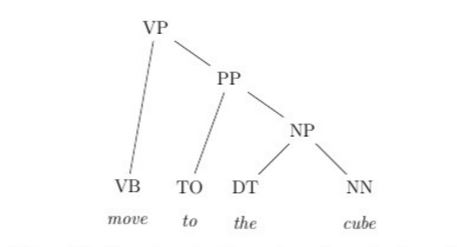
\includegraphics[width=0.45\textwidth]{parse_tree}
\caption{The parse tree for the command ``move to the cube''}
\label{fig:parse_tree}
\end{subfigure}
\vskip2ex
\begin{subfigure}[b]{\columnwidth}
\centering
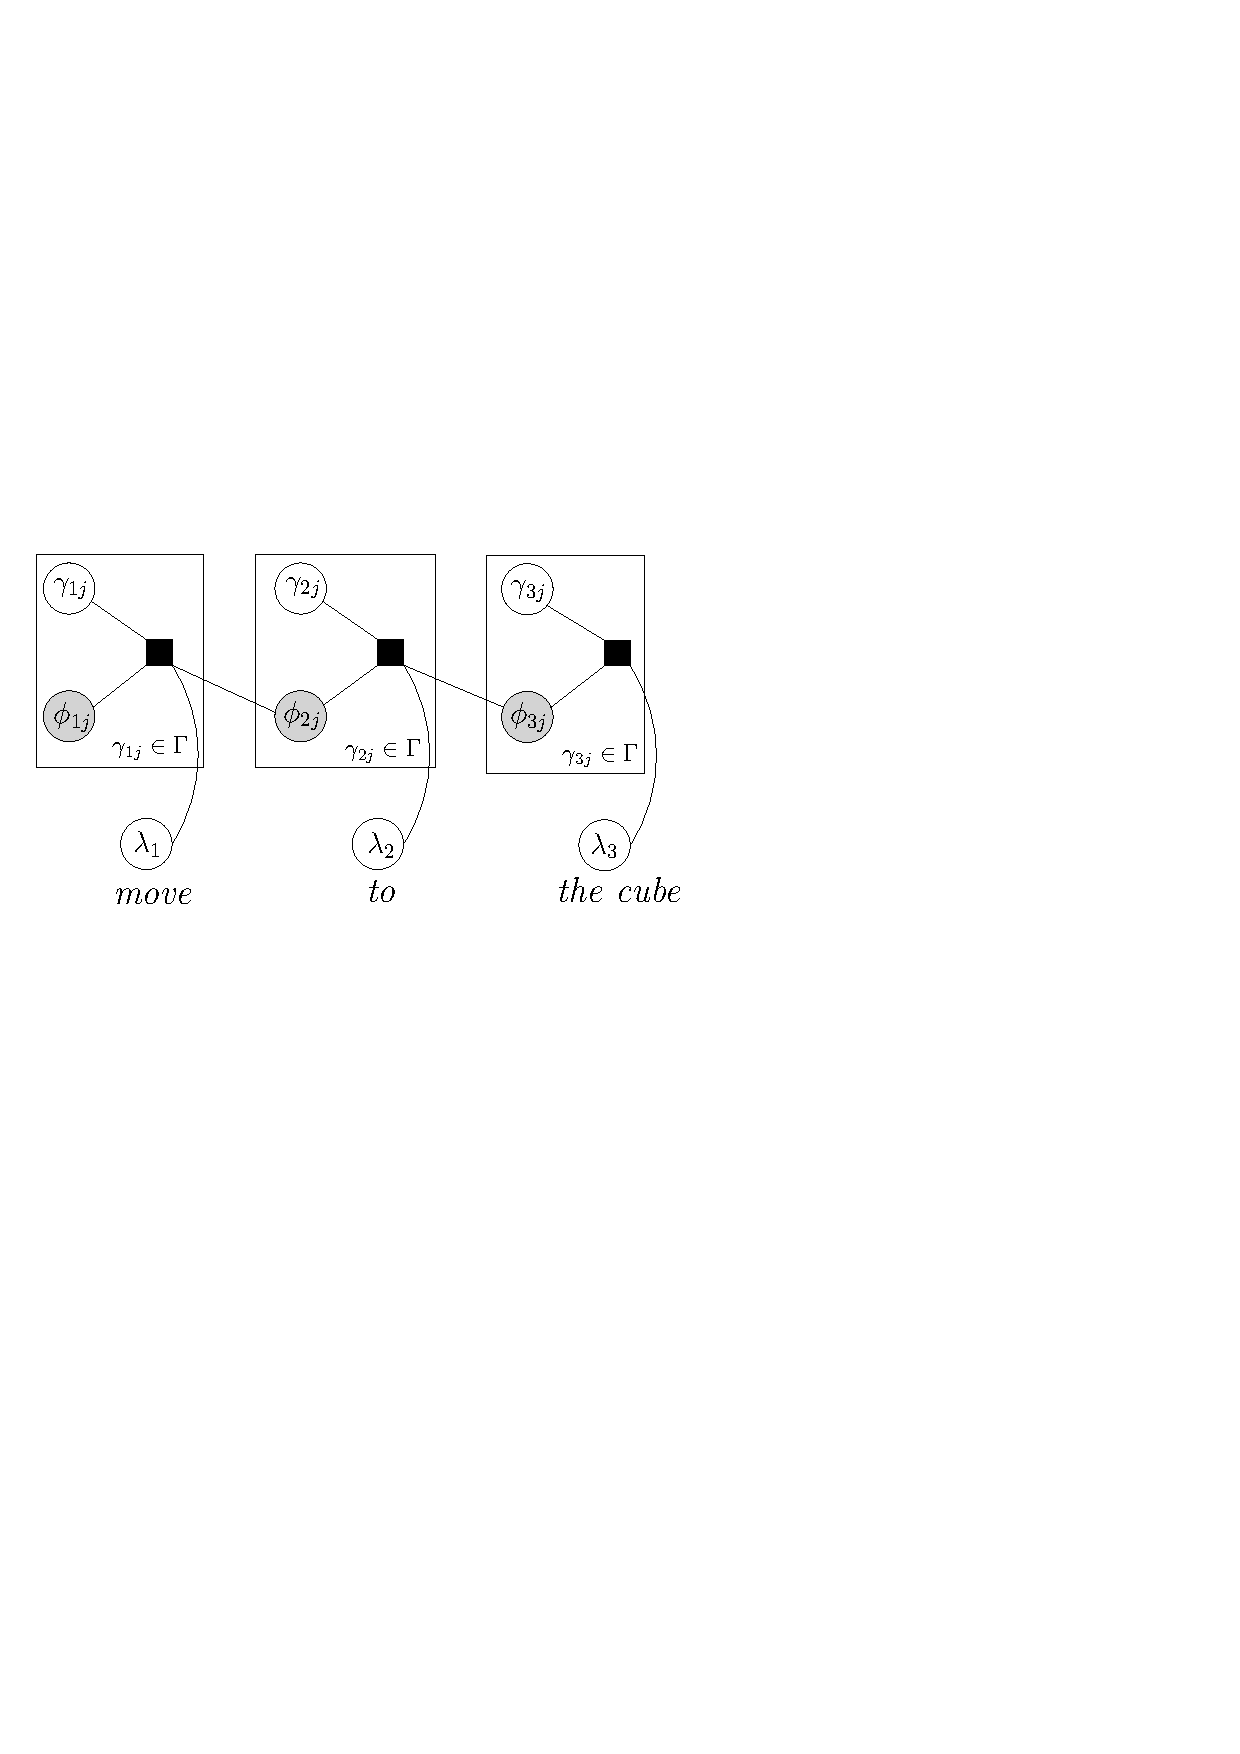
\includegraphics[width=0.7\textwidth]{dcg_plates_new.pdf}
\caption{The DCG graphical model for the parse tree in Fig.~\ref{fig:parse_tree}}
\label{fig:dcg_plates}
\end{subfigure}
\caption{An illustration of a parse tree and the corresponding DCG model where the graph topology of (b) is derived from the structure in (a). In the DCG model, the gray nodes are the observed variables (i.e., the correspondence variables), the white nodes in the plates are the unobserved variables (i.e., the grounding symbols), and the black nodes denote the factors (i.e., representing the conditional relationship between the variables)}
%\vskip-2.5ex
\end{figure}

Finally, the equation in \eqref{eq:dcg_factored1} can be factored as \eqref{eq:llm1}, where the factor function $\Psi : \Phi \times \Gamma \times \Lambda \times \Phi \times \Upsilon \rightarrow
 \mathbb{R}$ (e.g., within each plate in Fig.~\ref{fig:dcg_plates}) determines the most likely configuration $\boldsymbol{\phi^*}=\{\phi_{11}, \phi_{12}, \dots\}$ (where each $\phi_{ij} \in \Phi$) given $\gamma_{ij} \in \Gamma^i$, $\lambda_i \in \boldsymbol\lambda$, $\Phi_{c_{i}} \subset \Phi$, and $\Upsilon_{KP} \subset \Upsilon$. %Accordingly, one may rewrite \eqref{eq:dcg_factored1} as
%In order to expose the use of $\Psi$, one may rewrite Equation~\ref{eq:dcg_factored1} as Equation~\ref{eq:llm1}, \\
\begin{equation}
\boldsymbol{\phi}^* = \argmax_{\phi_{ij} \in \Phi} \prod_{i}^{\boldsymbol{|\lambda|}} \prod_{j}^{|\Gamma^i|} \Psi(\phi_{ij},\gamma_{ij},\lambda_i,\Phi_{c_{i}},\Upsilon_{KP}).
\label{eq:llm1}
\end{equation}

In \eqref{eq:llm1}, the factor function $\Psi$ is a log-linear model composed of a weighted combination of binary functions, that is,
\begin{equation}
\Psi(.) = \frac {\exp \Big( \sum\limits_{f \in F_{DCG}} \mu_f f(\phi_{ij},\gamma_{ij},\lambda_i,\Phi_{c_{i}},\Upsilon_{KP}) \Big)}{\sum\limits_{\phi_{ij} \in \{-1,0,1\}}\exp \Big( \sum\limits_{f \in F_{DCG}} \mu_f f(\phi_{ij},\gamma_{ij},\lambda_i,\Phi_{c_{i}},\Upsilon_{KP}) \Big)},
%\Psi(\phi_{ij},\gamma_{ij},\lambda_i,\Phi_{c_{i}},\Upsilon_{KP}) = \frac {\exp \Big( \sum\limits_{f \epsilon F} \mu_f f(\phi_{ij},\gamma_{ij},\lambda_i,\Phi_{c_{i}},\Upsilon_{KP}) \Big)}{\sum\limits_{\phi_{ij} \in \{-1,0,1\}}\exp \Big( \sum\limits_{f \epsilon F} \mu_f f(\phi_{ij},\gamma_{ij},\lambda_i,\Phi_{c_{i}},\Upsilon_{KP}) \Big)},
\label{eq:llm2}
\end{equation}
where $F_{DCG}$ is the set of hand-coded binary features that evaluate specific traits about a grounding. For example, a linguistic feature can express whether the word ``cube'' appears in the command $\boldsymbol{\lambda}$, or a geometric feature can identify the spatial characteristics of object aggregations (e.g., whether a region corresponds to the area between two objects). Moreover, each $f$ has a corresponding weight $\mu_f$. In the DCG model, the weights $\mu_f$ are learned by maximizing the training set likelihood using a stochastic gradient descent algorithm (i.e., the L-BFGS algorithm\footnote{In our work, we also use the {L-BFGS} algorithm to learn the weights of the feature functions} \cite{liu1989}). 

%  via learning,the weighting of each $f$. In this work,
%the weights $\mu_f$ are learned in a training procedure via .% to generate a more nuanced function that evaluates how likely a phrase is to correspond to a grounding.

Note that a limitation of the DCG model is that it assumes the set of symbols (i.e., objects and phrases) are defined a priori so it does not explicitly represent the unknown symbols. Thus, this model is unable to reason about objects and phrases that have not been trained on. 
\section{Probabilistic Model for Grounding Unknown Symbols} \label{sec:technical}
%In the previous section, it has been stated that the DCG model can be efficiently used in grounding problems where the objects and phrases are known and the phrases are grounded to only perceived objects. In this paper, the proposed model DCG-UPUP-Away enables the solution of a more generalized grounding problem such that 1) the phrases and objects may be known or unknown, and 2) the phrases may be grounded to objects that are out of perception. To this end, the following sections detail how to ground unknown phrases or objects, how to incrementally learn new objects and phrases, how to hypothesize groundings out of perception, and how to involve adjective attributes into grounding to avoid ambiguities.   

In this section, we extend the DCG model to infer unknown concepts. This is mainly achieved by introducing new symbols to the model. In the subsequent sections, we describe how to infer the grounding 1) unknown phrases or objects, and 2) hypothetical objects that are outside the robot's field of view. Then, we present a method to resolve ambiguities via linguistic context, which helps to improve the grounding performance of the proposed model.

\begin{figure*}
\centering
%\begin{subfigure}[t]{0.235\textwidth}
%\centering
%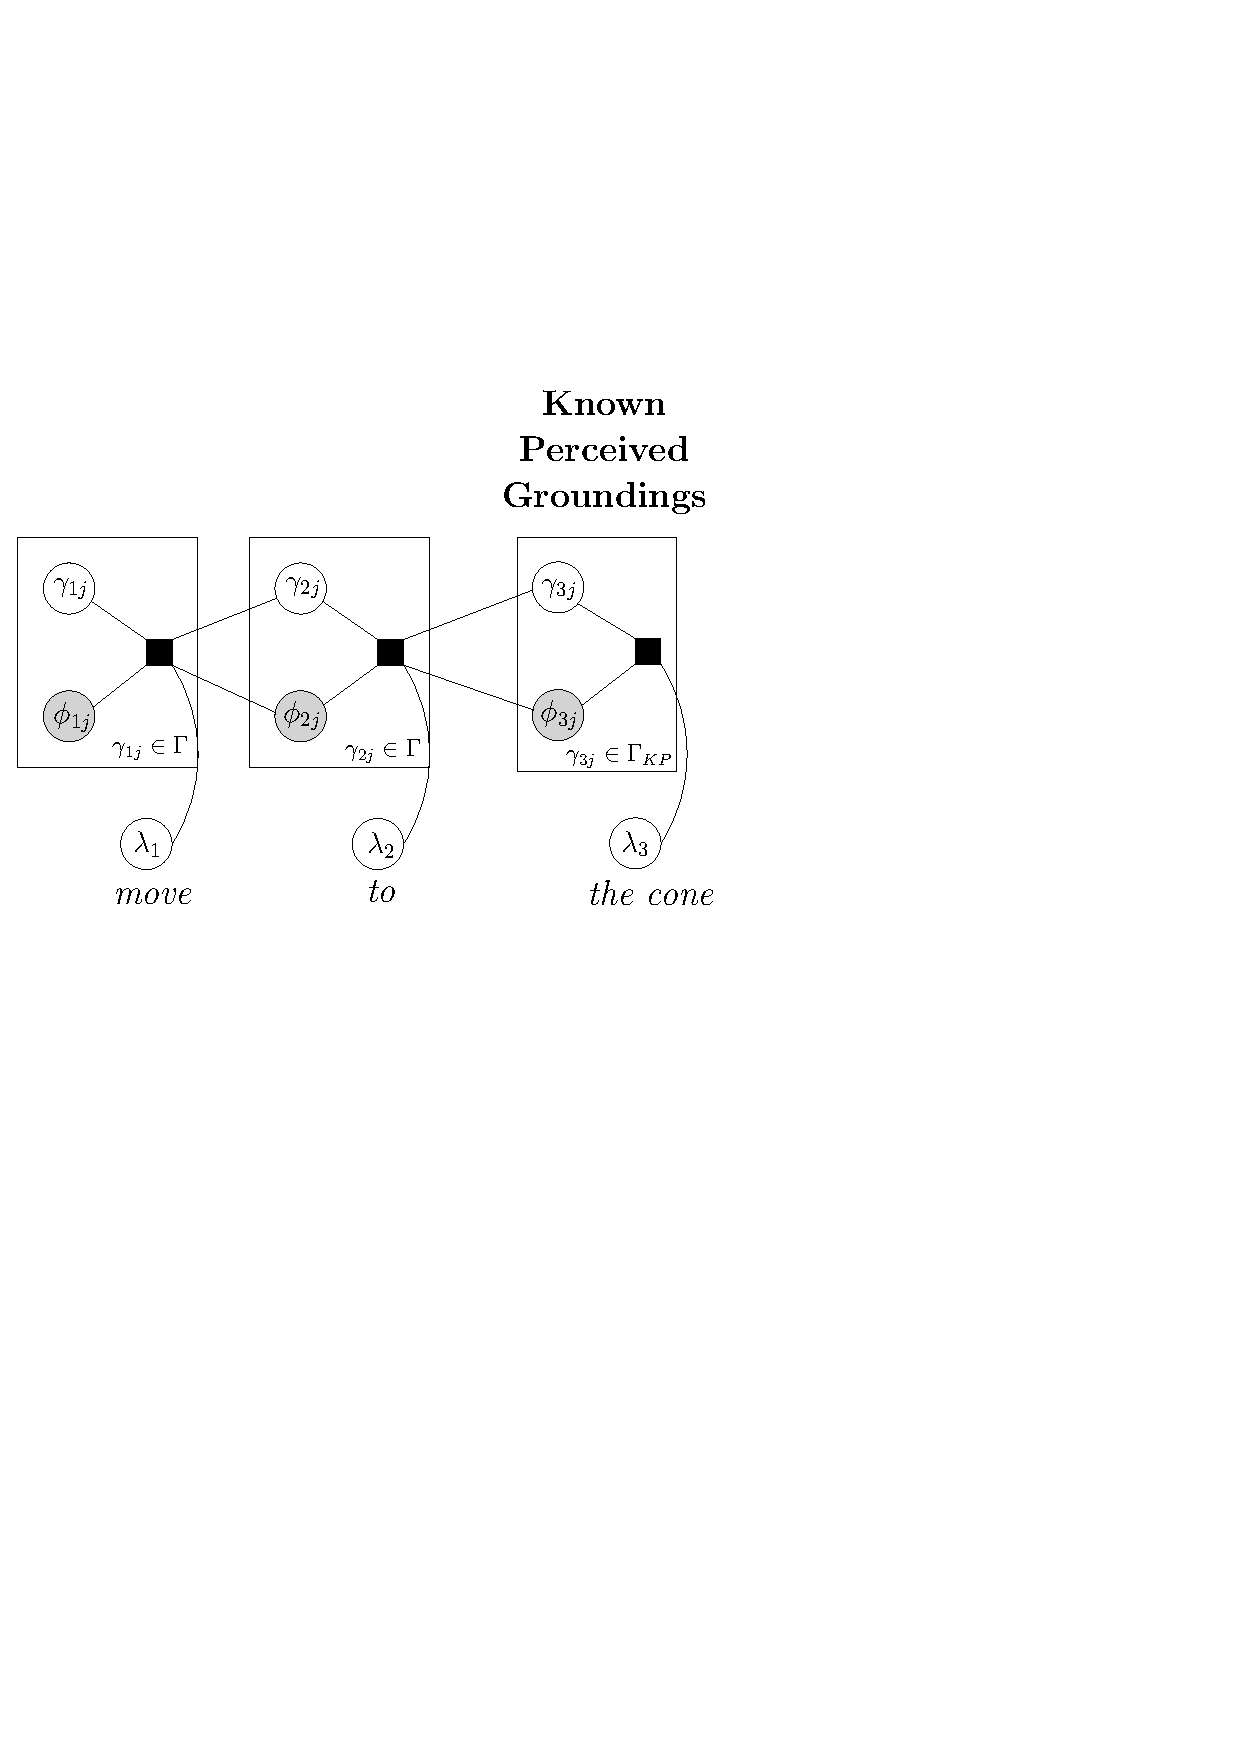
\includegraphics[width=\textwidth]{dcg.pdf}
%\caption{The DCG model}
%\label{fig:dcg}
%\end{subfigure}
%~
\begin{subfigure}[t]{0.40\textwidth}
\centering
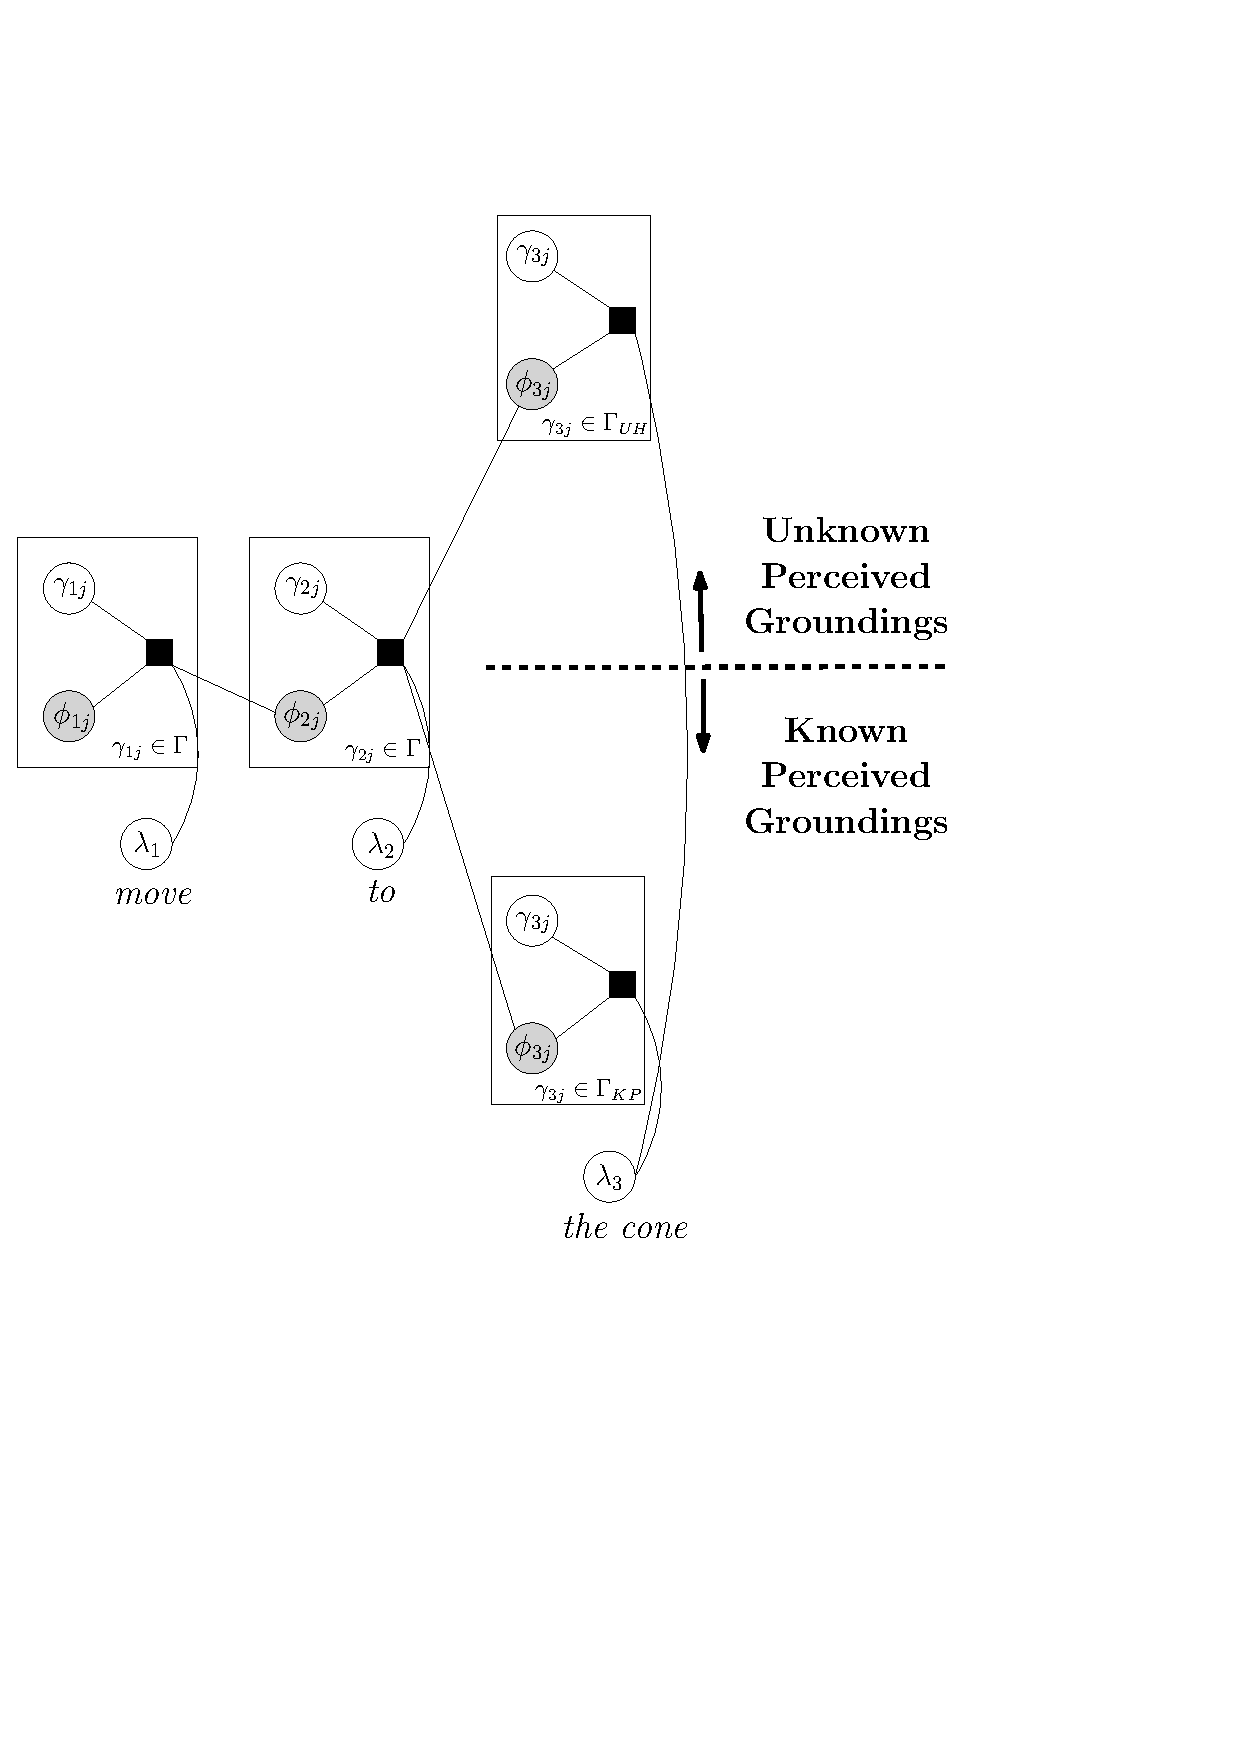
\includegraphics[width=\textwidth]{dcg_upup.pdf}
\caption{The DCG-UPUP model}
\label{fig:dcg-upup}
\end{subfigure}
~~~~
\begin{subfigure}[t]{0.52\textwidth}
\centering
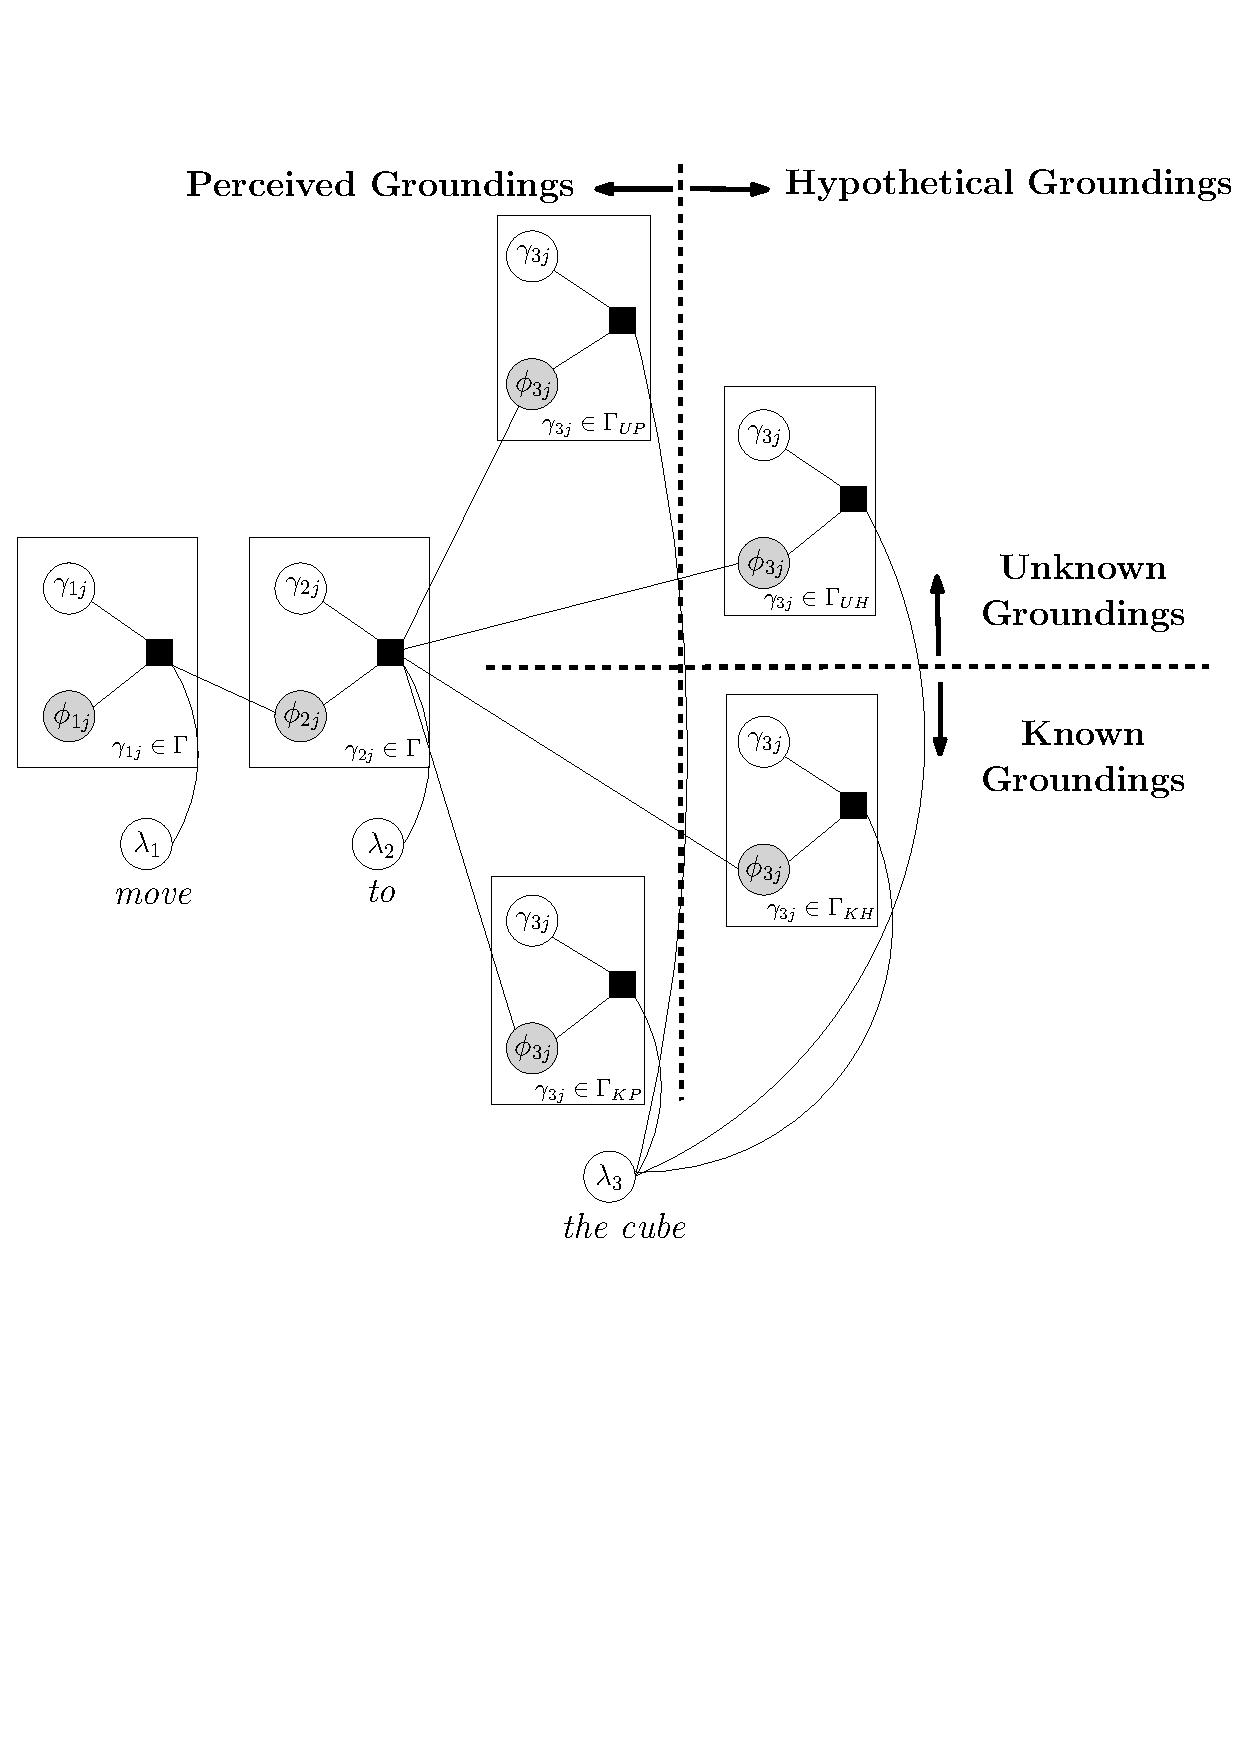
\includegraphics[width=\textwidth]{dcg_upup_away.pdf}
\caption{The DCG-UPUP-Away model}
\label{fig:dcg-upup-away}
\end{subfigure}
\caption{The graphical models instantiated for the command ``{move to the cube}". (a) The unknown groundings are explicitly represented and the grounding variables are assumed to be perceived. (b) The unknown perceived, known perceived, known hypothetical, and unknown hypothetical groundings are explicitly represented (separated by dashed lines).}
\end{figure*}

\subsection{Grounding Unknown Phrases or Objects}
%In this paper, the phrases (i.e., nouns) are
%defined as unknown if they have never grounded to a known
%object type in the training files. By maintaining a set of known
%nouns, one can easily determine whether or not a
%phrase is unknown. Similarly, the objects are defined as unknown
%if no object of the same class has ever appeared in the training
%data. 

%n this context, an object or a phrase is defined as unknown, if they have never appeared in the training. 

%An alternative model can be generated by decoupling the unknown symbols from the known symbols as in Fig.~\ref{fig:w_unknown} where each known symbol is connected to each unknown symbol (as dashed edges). While such a model represents all possible correlations between the known and unknown symbols, solving the grounding problem over this graph becomes computationally expensive due to strong connectivity.  

%Motivated by the idea of decoupling the unknown symbols from the known ones, we propose the DCG-UPUP model which exhibits a less connected graph than the one in Fig.~\ref{fig:w_unknown} (by removing the dashed edges). This simpler representation is mainly based on the following assumption: given the language command $\boldsymbol{\lambda}$ and the world model $\Upsilon$, the unknown groundings become conditionally independent from the known groundings because the variables $\boldsymbol\lambda$ and $\Upsilon$ are sufficient to predict the unknown groundings. 

In this work, a phrase is defined unknown if it has never been a part of a command in the training process. Similarly, an object is considered unknown, if it has never appeared in the world while training the model. The two main steps we take to enable grounding unknown phrases and objects are 1) to introduce a new grounding symbol to explicitly represent an unknown object and 2) to add new feature functions to identify whether an object or a phrase is unknown. Hence, the set of overall groundings can be defined as the union of unknown and known perceived groundings (i.e., $\Gamma = \Gamma_{UP} \cup \Gamma_{KP}$ \footnote{In the DCG model, $\Gamma = \Gamma_{KP}$.}), and the world model can be represented based on the known and unknown perceived objects as $\Upsilon = \Upsilon_{KP} \cup \Upsilon_{UP}$. The explicit representation of the unknown symbols is illustrated in Fig.~\ref{fig:dcg-upup}.

Similar to the DCG model assuming the conditional independence between the grounding variables, we assume that the known grounding variables are conditionally independent from the unknown grounding variables given the phrases. Note that this is illustrated in Fig.~\ref{fig:dcg-upup} by the absence of edges between the unknown and known symbols. Consequently, by using the new extended sets of groundings and the world model in \eqref{eq:llm1}, the factored  objective function for the DCG-UPUP model can be written as
\begin{equation}
\boldsymbol{\phi}^* = \argmax_{\phi_{ij} \in \boldsymbol{\phi}} \prod_{i}^{|\boldsymbol\lambda|} \prod_{j}^{|\Gamma^i_{KP} \cup \Gamma^i_{UP}|} \Psi(\phi_{ij},\gamma_{ij},\lambda_i, \Phi_{c_{i}},\Upsilon_{KP} \cup \Upsilon_{UP}).
\label{eq:dcg_upup_llm1}
\end{equation}

In addition to the set of linguistic or geometric feature functions $F_{DCG}$, in this work, we introduce a new set of binary feature functions, i.e., $F_U$, which identifies the unknown phrases and objects. For example, the identification of unknown phrases are achieved by keeping a list of known words, and then the corresponding feature $f$ checks whether a phrase in the command is in that list. On the other hand, the detection of unknown objects are realized by quantifying the classification likelihood (e.g., natural entropy \cite{grimmett2013}) of perceived objects based on the known object (image) classifiers. Accordingly, the factor function $\Psi(.)$ in \eqref{eq:dcg_upup_llm1} becomes a log-linear model with the new feature sets as follows: %by plugging the new extended sets of groundings and the features to \eqref{eq:llm1}, the factored objective function for the DCG-UPUP model can be written as      
%Motivated by the idea of decoupling the unknown symbols from the known ones, we propose an extension of the DCG model, that is the DCG-UPUP model, as illustrated in Fig.~\ref{fig:dcg-upup}. In light of going from \eqref{eq:dcg_factored1} to \eqref{eq:llm1}, the factored objective function for the DCG-UPUP model can be written as %in \eqref{eq:dcg_upup_llm1} where the the domain of the world model is extended to known and unknown perceived objects (i.e., $\Upsilon_{KP} \cup \Upsilon_{UP}$).
%where 
\begin{equation}
\Psi(.) = \frac{\exp \Big( \sum\limits_{f \in F_{\text{DCG}} \cup F_U} \mu_f f(\phi_{ij},\gamma_{ij},\lambda_i,\Phi_{c_{i}},\Upsilon_{KP} \cup \Upsilon_{UP}) \Big)}{\sum\limits_{\phi_{ij} \in \{0,1\}}\exp \Big( \sum\limits_{f \in F_{\text{DCG}} \cup F_U} \mu_f f(\phi_{ij},\gamma_{ij},\lambda_i,\Gamma_{c_{ij}},\Upsilon_{KP} \cup \Upsilon_{UP}) \Big)},
%\Psi(\phi_{ij},\gamma_{ij},\lambda_i,\Phi_{c_{i}},\Upsilon_{KP} \cup \Upsilon_{UP}) = \frac{\exp \Big( \sum_{f \in F_{\text{DCG}} \cup F_U} \mu_f f(\phi_{ij},\gamma_{ij},\lambda_i,\Phi_{c_{i}},\Upsilon_{KP} \cup \Upsilon_{UP}) \Big)}{\sum_{\phi_{ij} \in \{0,1\}}\exp \Big( \sum_{f \in F_{\text{DCG}} \cup F_U} \mu_f f(\phi_{ij},\gamma_{ij},\lambda_i,\Gamma_{c_{ij}},\Upsilon_{KP} \cup \Upsilon_{UP}) \Big)},
\label{eq:dcg_upup_llm2}
\end{equation}
%where
%\begin{equation}
%A_U= \exp \Big( \sum_{f \in F_{\text{DCG}} \cup F_U} \mu_f f(\phi_{ij},\gamma_{ij},\lambda_i,\Phi_{c_{i}},\Upsilon_{KP} \cup \Upsilon_{UP}) \Big) \nonumber
%%+ \sum_{f^\prime \in F_{U}} \mu_{f^\prime} f^\prime(\phi_{ij},\gamma_{ij},\lambda_i,\Phi_{c_{i}},\Upsilon_{KP} \cup \Upsilon_{UP}) \Big) \nonumber,
%\end{equation}
%
%\begin{equation}
%B_U= \sum_{\phi_{ij} \in \{0,1\}}\exp \Big( \sum_{f \in F_{\text{DCG}} \cup F_U} \mu_f f(\phi_{ij},\gamma_{ij},\lambda_i,\Gamma_{c_{ij}},\Upsilon_{KP} \cup \Upsilon_{UP}) \Big) \nonumber
%%+ \sum_{f^\prime \in F_{U}} \mu_{f^\prime} f^\prime(\phi_{ij},\gamma_{ij},\lambda_i,\Gamma_{c_{ij}},\Upsilon_{KP} \cup \Upsilon_{UP}) \Big), \nonumber
%\end{equation}
%%\exp \Big( \sum_{f \epsilon F_{\text{DCG}}} \mu_f f(\phi_{ij},\gamma_{ij},\lambda_i,\Gamma_{c_{ij}},\Upsilon_{KP} \cup \Upsilon_{UP}) \nonumber \\
%%\quad \quad \quad \quad \quad \quad \quad \quad \quad \quad \quad \quad 
%%+ \sum_{f \epsilon F_{\text{Unknown}}} \mu_f f(\phi_{ij},\gamma_{ij},\lambda_i,\Gamma_{c_{ij}},\Upsilon_{KP} \cup \Upsilon_{UP}) \Big)
%%\label{eq:dcg_upup_llm2}
%%\end{equation}
%$F_{DCG}$ and $F_{U}$ are the sets of hand-coded binary features used in the DCG model and for detecting unknown phrases or objects, respectively.
%\begin{figure}
%\centering
%\begin{subfigure}[t]{0.45\columnwidth}
%\centering
%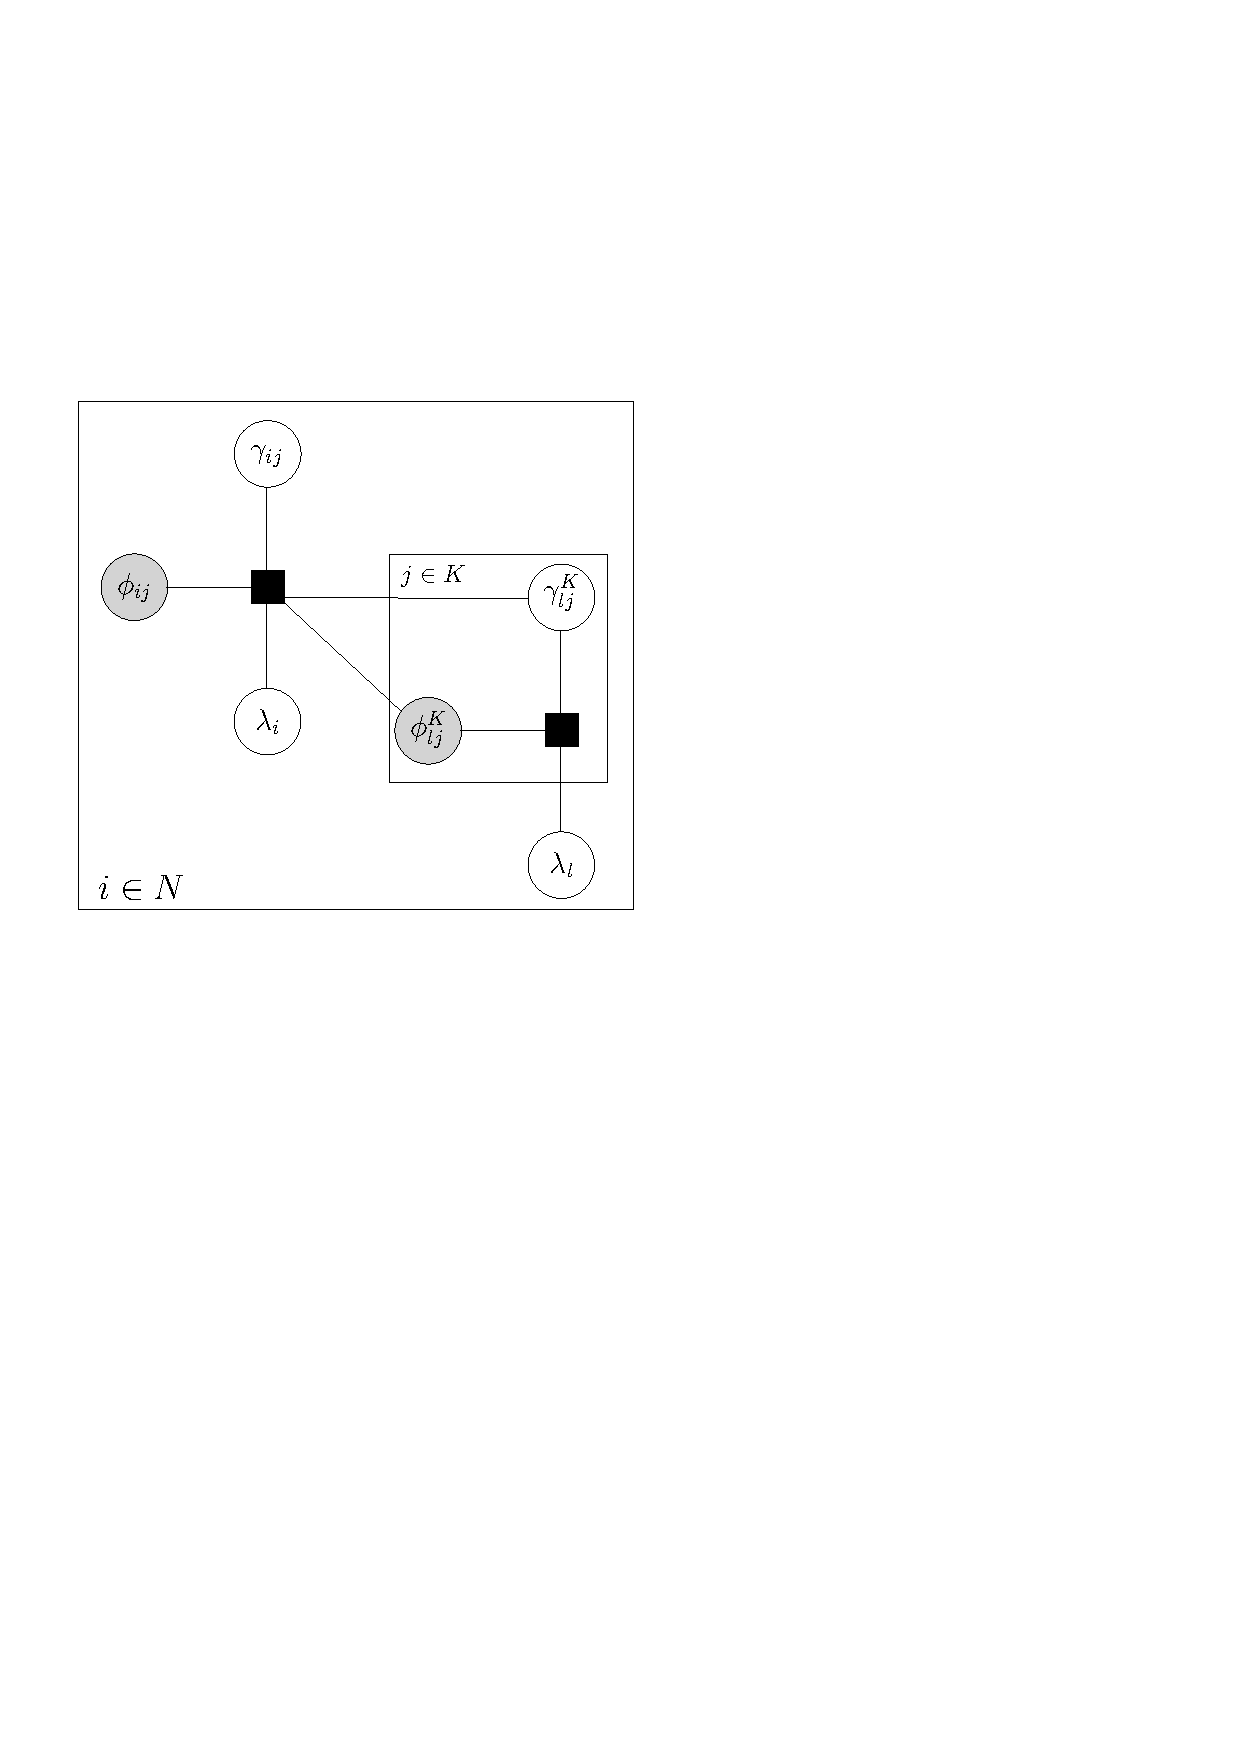
\includegraphics[width=\textwidth]{case1.pdf}
%\caption{Without explicit unknown grounding variables.}
%\label{fig:wo_unknown}
%\end{subfigure}
%~
%\begin{subfigure}[t]{0.51\columnwidth}
%\centering
%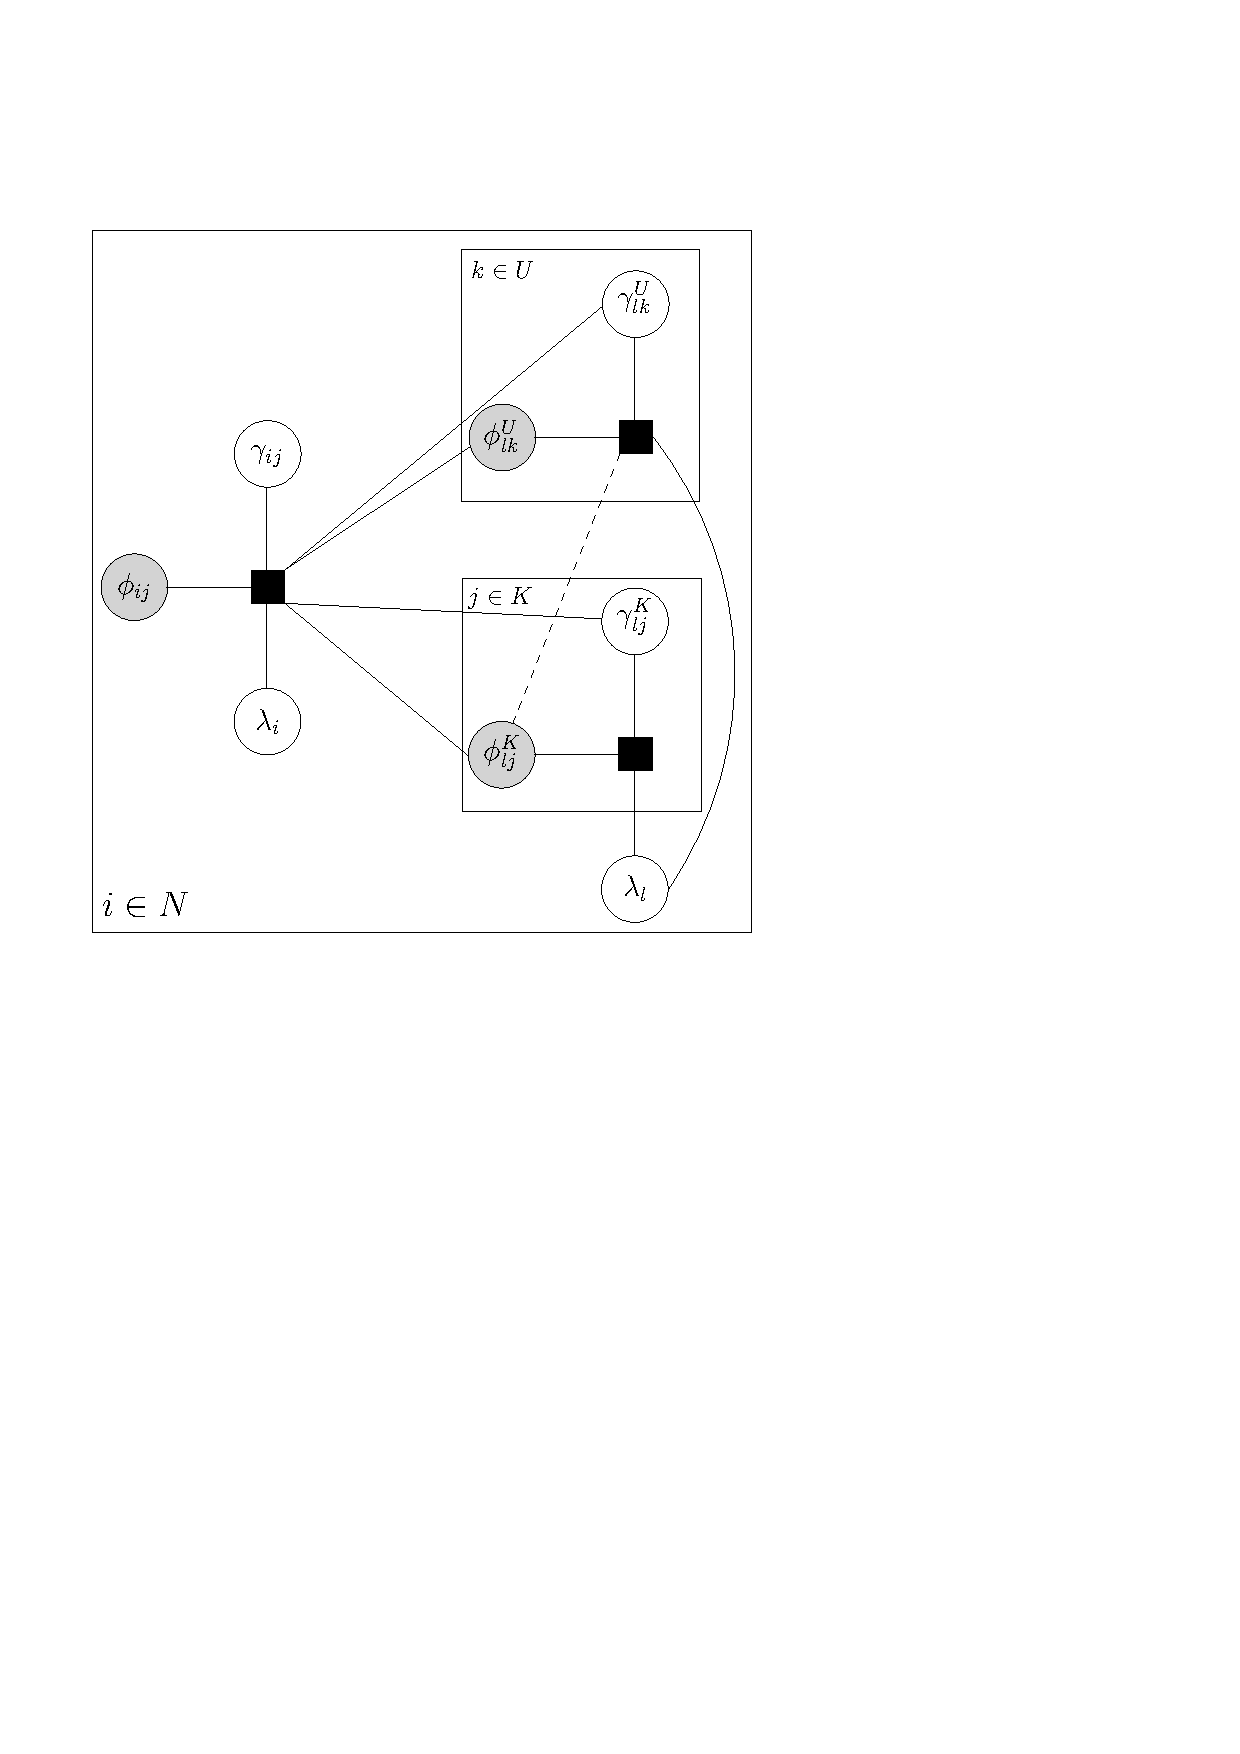
\includegraphics[width=\textwidth]{case2.pdf}
%\caption{With explicit unknown grounding variables.}
%\label{fig:w_unknown}
%\end{subfigure}
%
%\caption{Factor graph representations. Input instruction is parsed into $N$ phrases where $\lambda_l$ represents a child phrase of parent phrase $\lambda_i$. Superscripts $K$ and $U$ denote known and unknown variables, respectively.}
%\end{figure}

\subsection{Grounding Hypothetical Objects Outside the Field of View}
%The previous section presented that the DCG-UPUP model can explicitly represent the unknown phrases and objects. However, its performance is limited since the robot can only ground to the perceived objects. As an extension of this model, we introduce the DCG-UPUP-Away, which enables to ground phrases to objects that can be outside the field of view.
In this work, we define the hypothetical objects as the potential objects that can be located outside the robot's field of view. Now, we extend the DCG-UPUP model to enable grounding hypothetical objects. In existing models, the grounding is achieved based only on the objects that are perceived. However, a robot typically has a limited view of the world, and it is a strong assumption to consider that the given instructions always refer to the objects in the perceived world. To relax this assumption, we propose to add hypothetical objects to the model and let the robot associate a phrase with a hypothesized object when necessary.   

Adding hypothetical objects to the model is similar to the process of adding unknown objects to the model. First, after populating a world model by using the sensors of the robot, a single instance of every known object type, as well as one instance of an unknown object, are added to the world model and labeled as hypothetical objects. As a result, the new world model is composed of objects that are known perceived, unknown perceived, known hypothetical, and unknown hypothetical (i.e., $\Upsilon = \Upsilon_{KP} \cup \Upsilon_{UP} \cup \Upsilon_{KH} \cup \Upsilon_{UH}$). Second, new grounding symbols are added to explicitly represent the hypothetical objects. In a similar fashion, the set of groundings are extended as $\Gamma = \Gamma_{KP} \cup \Gamma_{UP} \cup \Gamma_{KH} \cup \Gamma_{UH}$. Third, a new set of binary features ($F_H$) is introduced to detect whether an object is hypothetical. For example, if the command contains an object that is not perceived based on the current field of view, then the referred object is considered hypothetical. Based on these modifications (the extensions of the world model $\Upsilon$, the grounding set $\Gamma$, and the feature functions $F$), the factored objective function for the DCG-UPUP-Away model can be written as
%As a comparison, Fig.~\ref{fig:dcg-upup} illustrates the DCG-UPUP model, where the nouns can be grounded to only known perceived and unknown perceived objects. Moreover, Fig.~\ref{fig:dcg} presents the DCG model where the nouns can be grounded to only known perceived objects.
%Similar to \eqref{eq:dcg_upup_llm1}, the factored objective function for the DCG-UPUP-Away model can be written by extending the world model to known perceived, unknown perceived, known hypothetical, and unknown hypothetical objects  (i.e., $\Upsilon_{KP} \cup \Upsilon_{UP} \cup \Upsilon_{KH} \cup \Upsilon_{UH}$) as follows:
\begin{equation}
\boldsymbol{\phi}^* = \argmax_{\phi_{ij} \in \boldsymbol{\phi}} \prod_{i}^{|\boldsymbol\lambda|} \prod_j^{|\bar\Gamma^i|} \Psi(\phi_{ij},\gamma_{ij},\lambda_i,\Phi_{c_{i}},\bar\Upsilon),
\label{eq:dcg_upup_away_llm1}
\end{equation}
where ${\bar{\Gamma}^i = \Gamma^i_{KP} \cup \Gamma^i_{UP} \cup \Gamma^i_{HP} \cup \Gamma^i_{HU}}$, $\bar\Upsilon = \Upsilon_{KP} \cup \Upsilon_{UP} \cup \Upsilon_{KH} \cup \Upsilon_{UH}$, and 
\begin{equation}
\Psi(.) = \frac{\exp \Big( \sum\limits_{f \in F_{\text{DCG}} \cup F_{U} \cup F_{H}} \mu_f f(\phi_{ij},\gamma_{ij},\lambda_i,\Gamma_{c_{ij}},\bar\Upsilon) \Big)}{\sum\limits_{\phi_{ij} \in \{0,1\}}\exp \Big( \sum\limits_{f \in F_{\text{DCG}} \cup F_{U} \cup F_{H}} \mu_f f(\phi_{ij},\gamma_{ij},\lambda_i,\Gamma_{c_{ij}},\bar\Upsilon) \Big)}.
\label{eq:dcg_upup_away_factor}
\end{equation}
%where
%\begin{equation}
%A_{UH}=\exp \Big( \sum_{f \in F_{\text{DCG}} \cup F_{U} \cup F_{H}} \mu_f f(\phi_{ij},\gamma_{ij},\lambda_i,\Gamma_{c_{ij}},\Upsilon_{KP} \cup \Upsilon_{UP} \cup \Upsilon_{KH} \cup \Upsilon_{UH}) \Big) \nonumber
%%\quad \quad \quad \quad \quad \quad + \sum_{f' \in F_{U}} \mu_{f'} f'(\phi_{ij},\gamma_{ij},\lambda_i,\Gamma_{c_{ij}},\Upsilon_{KP} \cup \Upsilon_{UP} \cup \Upsilon_{KH} \cup \Upsilon_{UH}) \nonumber \\
%%\quad \quad \quad \quad \quad \quad + \sum_{f^{\prime\prime} \in F_{H}} \mu_{f^{\prime\prime}} f^{\prime\prime}(\phi_{ij},\gamma_{ij},\lambda_i,\Gamma_{c_{ij}},\Upsilon_{KP} \cup \Upsilon_{UP} \cup \Upsilon_{KH} \cup \Upsilon_{UH}) \Big), \nonumber
%\end{equation}
%
%\begin{equation}
%B_{UH}=\sum_{\phi_{ij} \in \{0,1\}}\exp \Big( \sum_{f \in F_{\text{DCG}} \cup F_{U} \cup F_{H}} \mu_f f(\phi_{ij},\gamma_{ij},\lambda_i,\Gamma_{c_{ij}},\Upsilon_{KP} \cup \Upsilon_{UP} \cup \Upsilon_{KH} \cup \Upsilon_{UH}) \Big) \nonumber
%%\quad \quad \quad \quad \quad \quad \quad \quad + \sum_{f' \in F_{U}} \mu_{f'} f'(\phi_{ij},\gamma_{ij},\lambda_i,\Gamma_{c_{ij}},\Upsilon_{KP} \cup \Upsilon_{UP} \cup \Upsilon_{KH} \cup \Upsilon_{UH}) \nonumber \\
%%\; \quad \quad \quad \quad \quad \quad \quad \quad + \sum_{f^{\prime\prime} \in F_{H}} \mu_{f^{\prime\prime}} f^{\prime\prime}(\phi_{ij},\gamma_{ij},\lambda_i,\Gamma_{c_{ij}},\Upsilon_{KP} \cup \Upsilon_{UP} \cup \Upsilon_{KH} \cup \Upsilon_{UH}) \Big), \nonumber
%\end{equation}
%and $F_H$ is the set of hand-coded binary features to detect if an object is hypothetical. 
%\color{black}

Note that the resulting graphical model for the DCG-UPUP-Away is illustrated in Fig.~\ref{fig:dcg-upup-away}, where the nouns may ground to 1) known and perceived objects, 2) unknown and perceived objects, 3) known and hypothetical objects, and 4) unknown and hypothetical objects. 
\subsection{Resolving Ambiguity via Linguistic Context}
\label{sec:color}
In real-world applications, there might exist multiple objects with the same type but different attributes. In order to resolve the ambiguities among the objects, it is crucial to allow the association between the natural language adjectives and the object properties. For example, if there exist two cube type objects in the world, one way to distinguish them from each other is to consider their properties such as color or size. In this section, we present how to include color information into the solution of grounding problem over the DCG-UPUP-Away \footnote{Other attributes such as size or shape can be included in a similar way by adding the corresponding feature functions.}. To this end, a new set of feature functions is introduced, that is $F_C = \{f_{color}, f_{word}\}$ where the feature $f_{color}$ expresses the color property of an object (e.g., whether the cube is red or not) and the feature $f_{word}$ identifies whether the language command $\boldsymbol\lambda$ contains a color adjective. Note that the addition of new features brings only a minor change to \eqref{eq:dcg_upup_away_factor} where the set of features are extended, i.e, $f \in F_{DCG} \cup F_U \cup F_H \cup F_C$. 

%One way to improve the grounding performance of the DCG-UPUP-Away model is to allow the association between the natural language adjectives and the object properties. For example, if there exist two cube type objects in the world, one way to distinguish them from each other is to consider their properties such as color or size. In this section, we present how to include color information into the solution of grounding problem over the DCG-UPUP-Away \footnote{Other attributes such as size or shape can be included in a similar way by adding the corresponding feature functions.}. To this end, a new set of feature functions is introduced, that is $F_C = \{f_{color}, f_{word}\}$ where the feature $f_{color}$ checks the color property of an object and the feature $f_{word}$ detects whether the language command $\boldsymbol\lambda$ contains a color adjective. Note that the addition of new features brings only a minor change to \eqref{eq:dcg_upup_away_factor} where the set of features are extended, i.e, $f \in F_{DCG} \cup F_U \cup F_H \cup F_C$. 

%each feature function $\Psi(.)$ is defined as follows:
%\begin{equation}
%\Psi(\phi_{ij},\gamma_{ij},\lambda_i,\Gamma_{c_{ij}},\Upsilon_{KP} \cup \Upsilon_{UP} \cup \Upsilon_{KH} \cup \Upsilon_{UH}) = \frac{A_{UHC}}{B_{UHC}}
%\label{eq:color_llm2}
%\end{equation}
%where
%\begin{equation}
%A_{UHC}=\exp \Big( \sum_{f \in F_{\text{DCG}}} \mu_f f(\phi_{ij},\gamma_{ij},\lambda_i,\Gamma_{c_{ij}},\Upsilon_{KP} \cup \Upsilon_{UP} \cup \Upsilon_{KH} \cup \Upsilon_{UH}) \nonumber \\
%\quad \quad \quad \quad \quad \quad + \sum_{f' \in F_{U}} \mu_{f'} f'(\phi_{ij},\gamma_{ij},\lambda_i,\Gamma_{c_{ij}},\Upsilon_{KP} \cup \Upsilon_{UP} \cup \Upsilon_{KH} \cup \Upsilon_{UH}) \nonumber \\
%\quad \quad \quad \quad \quad \quad + \sum_{f^{\prime\prime} \in F_{H}} \mu_{f^{\prime\prime}} f^{\prime\prime}(\phi_{ij},\gamma_{ij},\lambda_i,\Gamma_{c_{ij}},\Upsilon_{KP} \cup \Upsilon_{UP} \cup \Upsilon_{KH} \cup \Upsilon_{UH}) \nonumber \\
%\quad \quad \quad \quad \quad \quad + \sum_{f^{\prime\prime\prime} \in F_{C}} \mu_{f^{\prime\prime\prime}} f^{\prime\prime\prime}(\phi_{ij},\gamma_{ij},\lambda_i,\Gamma_{c_{ij}},\Upsilon_{KP} \cup \Upsilon_{UP} \cup \Upsilon_{KH} \cup \Upsilon_{UH}) \Big), \nonumber
%\end{equation}
%
%\begin{equation}
%B_{UHC}=\sum_{\phi_{ij} \in \{0,1\}}\exp \Big( \sum_{f \in F_{\text{DCG}}} \mu_f f(\phi_{ij},\gamma_{ij},\lambda_i,\Gamma_{c_{ij}},\Upsilon_{KP} \cup \Upsilon_{UP} \cup \Upsilon_{KH} \cup \Upsilon_{UH}) \nonumber \\
%\quad \quad \quad \quad \quad \quad \quad \quad + \sum_{f' \in F_{U}} \mu_{f'} f'(\phi_{ij},\gamma_{ij},\lambda_i,\Gamma_{c_{ij}},\Upsilon_{KP} \cup \Upsilon_{UP} \cup \Upsilon_{KH} \cup \Upsilon_{UH}) \nonumber \\
%\quad \quad \quad \quad \quad \quad \quad \quad + \sum_{f^{\prime\prime} \in F_{H}} \mu_{f^{\prime\prime}} f^{\prime\prime}(\phi_{ij},\gamma_{ij},\lambda_i,\Gamma_{c_{ij}},\Upsilon_{KP} \cup \Upsilon_{UP} \cup \Upsilon_{KH} \cup \Upsilon_{UH})\nonumber \\
%\; \quad \quad \quad \quad \quad \quad \quad \quad + \sum_{f^{\prime\prime\prime} \in F_{C}} \mu_{f^{\prime\prime\prime}} f^{\prime\prime\prime}(\phi_{ij},\gamma_{ij},\lambda_i,\Gamma_{c_{ij}},\Upsilon_{KP} \cup \Upsilon_{UP} \cup \Upsilon_{KH} \cup \Upsilon_{UH}) \Big), \nonumber
%\end{equation}
%and $F_C$ is the set of hand-coded binary features for detecting color phrases or properties (i.e., $F_C = f_{color} \cup f_{word}$).


\section{Online Learning}
\label{sec:implementation}
In this section, we propose an unsupervised online learning strategy for the model to acquire new symbols. To this end, we present an exploration phase for the robot to search for unknown objects and an incremental learning strategy to learn new symbols.
\subsection{Exploration to Find an Unknown Object}
Given a natural language command, a robot can ground the phrases within its world model by solving an inference problem over the DCG-UPUP-Away model. Consequently, a noun phrase can be grounded to a perceived (known or unknown) or a hypothetical (known or unknown) object. In the case of grounding to a hypothetical object, the robot needs to explore its surroundings to find the potential object that is referred by the phrase. There might be several exploration strategies to find the hypothetical object. In this work, we assume that the robot gradually rotates in its current position to change its field of view. As the field of view changes, the world model is updated based on the new perceived objects, and the grounding problem with the same command is solved over the DCG-UPUP-Away model until the noun phrase is grounded to a perceived object.   


\subsection{Incremental Unsupervised Learning}
Suppose that a robot is given a command with an unknown phrase. The solution over the DCG-UPUP-Away model is the association of the unknown phrase with the unknown object in the environment. When the robot perceives an unknown object as it is initially deployed, then the unknown phrase grounds to that unknown object. If the world model in its initial deployment does not contain an unknown object, it starts to explore the environment (as discussed in the previous section). Whenever it finds an unknown object, then the unknown phrase is grounded to that object. 

In addition to grounding unknown phrases to unknown objects, the model is capable of learning new symbols (objects and phrases) based on the past experience. In that case, although a robot starts a mission with a small set of known phrases and objects, it can incrementally increase its knowledge on phrases and objects and perform more efficiently in the future. To achieve this, whenever an unknown phrase is grounded to an unknown object, we propose an unsupervised learning procedure with the following steps: 
%Consequently, the unknown phrases can be grounded to unknown objects In the case of grounding to an unknown perceived object (either initially or after exploring the environment), the DCG-UPUP-Away model can reason about the corre
%While the DCG-UPUP model can reason about unknown phrases and objects, it can also learn new symbols permanently. This is mainly achieved by the following unsupervised learning procedure: whenever an unknown phrase is grounded to an unknown object, a new type is created based on the new phrase. Then, a new training example, in which the phrase grounds to the new
%type, is generated. Accordingly, the LLM models are retrained with the expanded set of training examples. Consequently, when the newly generated objects (or phrases) are encountered again, they become known symbols. Hence, the DCG-UPUP model can learn to associate a new phrase with a new type.
\vskip0.5ex
\noindent \emph{Step 1:} A new object type is created. For example, if the unknown noun phrase is "apple", a new symbolic apple-type object is created.
\vskip0.5ex
\noindent \emph{Step 2:} Based on the given command, the current world model, and the grounding solution, a new training file is created. For example, suppose that the world contains one apple, one cube, and one cone, and the robot initially knows what a cube and cone are. Let the command be ``go near the apple". Then, the DCG-UPUP-Away model will correspond to the unknown phrase ``apple" with the unknown object apple. After creating the new object type for apple as in step 1, the grounding solution is updated as corresponding the phrase ``apple" with the apple-type object. Consequently, the current world model, the given command, and the updated grounding solution constitute a new training file.
\vskip0.5ex
\noindent \emph{Step 3:} Since a new object type is created (e.g., apple-type), the set of groundings ($\Gamma$) is updated by adding the new symbolic object. 
\vskip0.5ex
\noindent \emph{Step 4:}  Since a new object type is added and an unknown phrase is grounded (from step 3), the set of features are updated as follows: first, a new feature function is created to classify whether an object corresponds to the new type. For example, several images of the apple are taken and an apple classifier is trained. Accordingly, the feature function returns true if an object is likely to be an apple based on the classifier. Second, the feature function to check whether a word is known is updated (e.g., the phrase ``apple" is added to the list of known words). 
\vskip0.5ex

Consequently, after creating a new training file and updating the set of groundings and the feature functions, the log linear model in \eqref{eq:dcg_upup_away_factor} is retrained to update the weighting functions. Hence, initially unknown symbols become known after the training.  


%\begin{algorithm}[b!]\footnotesize
%\caption{Grounding/Learning over DCG-UPUP-Away}\label{alg:dcg_upup_away}
%\begin{algorithmic}[1]
%\Procedure{DCG-UPUP-Away}{}
%\State $M \gets \text{new DCG-UPUP-Away}$
%\State $M.\Gamma \gets \text{init\_groundings}$
%\State $M.F \gets \text{init\_features}$
%\State $T \gets \text{init\_training}$
%\State $M.\text{train}(M.\Gamma, M.F, T)$
%\While {true}
%\State $\Upsilon \gets \text{perceive\_objects}(\text{camera},M.\Gamma)$
%\State $\Upsilon \gets \Upsilon + \text{hypothesize\_objects}(M.\Gamma)$
%\State $\boldsymbol{\lambda} \gets \text{get\_nl\_command}()$
%\State $[\boldsymbol{\phi}^*,\boldsymbol{\gamma}^*] \gets M.\text{ground}(\boldsymbol{\lambda},\Upsilon)$
%\If {$\boldsymbol{\gamma}^*.\text{is\_hypothesized}()$}
%\State $\text{explore\_surroundings()}$
%\Else
%\State $\text{drive\_to}(\boldsymbol{\gamma}^*)$
%\EndIf
%\State $T_u \gets \text{gen\_unsupervised\_training}(\boldsymbol{\lambda},\boldsymbol{\gamma}^*,\Upsilon)$
%\If {$\text{is\_unknown}(\boldsymbol{\lambda}) \& !\boldsymbol{\gamma}^*.\text{is\_hypothesized}()$}
%\State $\gamma' \gets \text{new\_grounding}(\boldsymbol{\lambda},\boldsymbol{\gamma}^*,\Upsilon)$
%\State $M.\Gamma \gets M.\Gamma + \gamma'$
%\State $M.F \gets M.F + f_{\text{word}}(\boldsymbol{\lambda}[\text{noun}])$
%\State $M.F \gets M.F + f_{\text{color}}(\boldsymbol{\gamma}^*[\text{color}])$
%\State $M.F \gets M.F + f_{\text{obj}}(\boldsymbol{\gamma}^*[\text{obj}])$
%\State $T_u \gets \text{replace\_unknown}(T_u,\gamma')$
%\EndIf
%\State $T \gets T + T_u$
%\State $M.\text{train}(M.\Gamma, M.F, T)$
%\EndWhile
%\EndProcedure
%\end{algorithmic}
%\end{algorithm}
%\subsection{Overview of the Pseudo-code}

%The pseudo-code for grounding and learning new symbols over the DCG-UPUP-Away model is presented in Alg.~\ref{alg:dcg_upup_away}. First, the graphical model $M$ is initialized and trained with the initial set of training data (lines 1-6). Grounding to unknown symbols and/or hypothetical objects are tackled between the lines 7-24. In particular, the world model is updated with the perceived objects (line~8) and then hypothetical objects are added (line~9). The natural language command is entered as an input (line~10). Using the model $M$ with the language command $\boldsymbol\lambda$ and the most recent world model $\Upsilon$, the grounding problem is solved (line~11). If the obtained grounding is hypothetical, then the robot initiates the exploration (line~13); otherwise the robot moves towards the grounded perceived object (line~15). Note that the exploration in this research is considered as the robot rotating in its current location. At the end of solving the grounding problem, a new training file is generated based on the given command $\boldsymbol\lambda$, the resulting grounding $\boldsymbol\gamma^*$, and the current world model $\Upsilon$ (line~16). If there exists an unknown phrase in the given command and the resulting grounding is not hypothetical, then a new object type (or grounding variable) is generated (line~18) and the set of grounding variables as well as the feature sets are updated (lines~19-22). Finally, the newly generated object type $\gamma^\prime$ replaces the unknown object type in training file $T_u$ (line~23), and the model $M$ is retrained with the new set of training data. Consequently, the initially unknown object becomes a known object in the new model $M$ in the further iterations. 



%\begin{equation}
%\Psi() = \exp \Big( \sum_{f \epsilon F_{\text{DCG}}} \mu_f f(\phi_{ij},\gamma_{ij},\lambda_i,\Gamma_{c_{ij}},\Upsilon_{KP} \cup \Upsilon_{UP} \cup \Upsilon_{KH} \cup \Upsilon_{UH}) +...\\
%\sum_{f' \epsilon F_{\text{Unknown}}} \mu_{f'} f'(\phi_{ij},\gamma_{ij},\lambda_i,\Gamma_{c_{ij}},\Upsilon_{KP} \cup \Upsilon_{UP} \cup \Upsilon_{KH} \cup \Upsilon_{UH}) +...\\
%\mu_{f_H} f_{H}(\phi_{ij},\gamma_{ij},\lambda_i,\Gamma_{c_{ij}},\Upsilon_{KP} \cup \Upsilon_{UP} \cup \Upsilon_{KH} \cup \Upsilon_{UH}) +...\\
%\sum_{f'' \epsilon F_{\text{Color}}} \mu_{f''} f''(\phi_{ij},\gamma_{ij},\lambda_i,\Gamma_{c_{ij}},\Upsilon_{KP} \cup \Upsilon_{UP} \cup \Upsilon_{KH} \cup \Upsilon_{UH}) \Big)
%\label{eq:color_llm2}.
%\end{equation}

\section{Evaluation}
\label{sec:evaluation}
The performance of the DCG-UPUP-Away model is demonstrated in two experiments.
First, a simulated turtlebot within randomly generated simulated environments is given a series of user-generated natural language commands.
Second, an actual turtlebot is given specific commands in a laboratory environment in order to demonstrate novel behaviors enabled by the DCG-UPUP-Away model.
Both experiments assume a perfect object recognizer that translates the raw sensor data into a world model $\Upsilon$ that can be used by the DCG-UPUP-Away model, as well as an initial set of hand-labeled training examples for training the LLM to ground cubes, spheres, and cylinders.
In all trials, training the model with $53$ positive examples took less than $1$ minute on a Lenovo Thinkpad X1 Carbon, and grounding a command took under $40$ seconds.
\subsection{Experimental Setup}
The simulated testing environments are randomly generated in Gazebo.
Ten worlds are created, and each is populated with a random collection of objects in randomized locations.
There are $8$ possible object types (including cubes, spheres, and cylinders) in $3$ possible colors, for a total of $24$ objects.
Each object has a $15\%$ chance of being added to a given map.
Using such a procedure to generate environments coupled with the limited field of view of the turtlebot has caused $87\%$ of the objects to be placed outside the initial field of view of the robot, which demonstrates the need for the ability to ground commands to hypothesized objects.

After generating the 10 worlds, the screenshots of a world with a highlighted single object are uploaded to Amazon Mechanical Turk. For each image, the users were instructed to write a command ``for approaching the highlighted object.''
These image-command pairs were saved for evaluating whether a robot, when placed in the corresponding simulated world and given the natural language command, successfully approaches the correct object.
An example screenshot, with an annotation supplied by a user, is shown in Fig.~\ref{fig:amt}.
\begin{figure}[h]
	\centering
    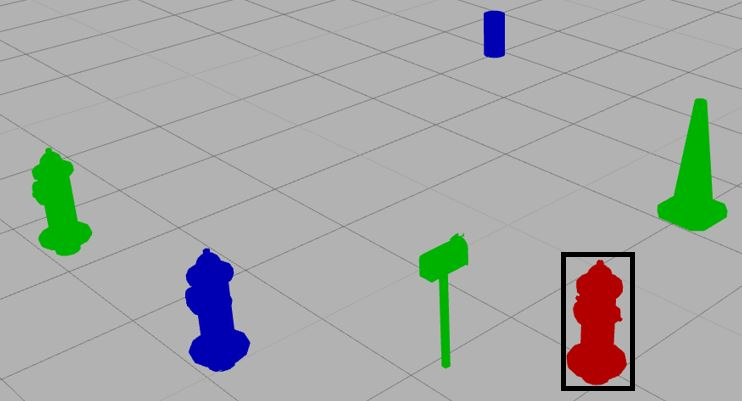
\includegraphics[width=7.8cm]{amt}
	\caption{A simulated world with a highlighted object presented on Amazon Mechanical Turk, labeled by a user as ``Move to the red fire hydrant.''}
	\label{fig:amt}
\end{figure}

Ten image-command pairs are randomly selected without any replacement from the pool of all pairs.
Note that a trial along the paper refers to $10$ ordered pairs, and each specific pair is called one iteration.
Accordingly, $30$ trials are generated, each consisting of $10$ iterations, for a total of $300$ evaluations.
When executing a trial, the turtlebot is first trained on the initial, hand-curated training set.
The turtlebot is then given the natural language command from the first iteration, and then retrained using the initial data supplemented by unsupervised training examples generated by the first iteration.
The retrained turtlebot is given the command from the next iteration, and appropriately retrained after each execution until all 10 iterations have been executed.

The metrics we consider for the performance of the model are the grounding accuracy (how likely the DCG-UPUP-Away model correctly grounds a phrase) and the number of known symbols.
We further divide the grounding accuracy results to examine when phrases are grounded to known, unknown, or learned objects.
\subsection{Grounding Accuracy}
%The primary metric used in evaluating the success of DCG-UPUP-Away is the grounding accuracy: how likely is the turtlebot to correctly execute the natural language command.
As discussed previosuly, the turtlebot is retrained between iterations, thus the grounding accuracy may change as a function of iteration number. In fact, the mean grounding accuracy remains between $70\%$ and $90\%$ across all iterations, as shown in Figure~\ref{fig:g_acc}. Although the overall grounding accuracy remains relatively constant, the underlying behavior within the DCG-UPUP-Away model changes over the course of a trial. For example, Fig.~\ref{fig:g_acc_split} illustrates 3 curves showing what fraction of correctly grounded phrases refer to known objects, unknown objects, or learned objects as a function of iteration number. In the first iteration, nearly $70\%$ of correctly grounded commands refer to known objects, but by the 10$^\text{th}$ iteration that number has fallen to nearly $10\%$, replaced almost entirely by correctly grounding to learned objects.

\begin{figure}[h!]
\begin{subfigure}[b]{0.47\columnwidth}
\centering
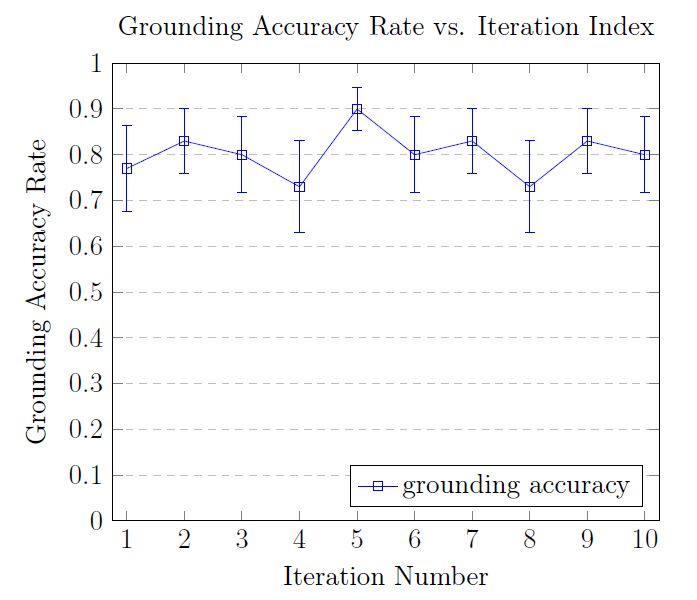
\includegraphics[width=\textwidth]{g_acc}
\caption{Overall grounding accuracy.}
\label{fig:g_acc}
\end{subfigure}
~
\begin{subfigure}[b]{0.50\columnwidth}
\centering
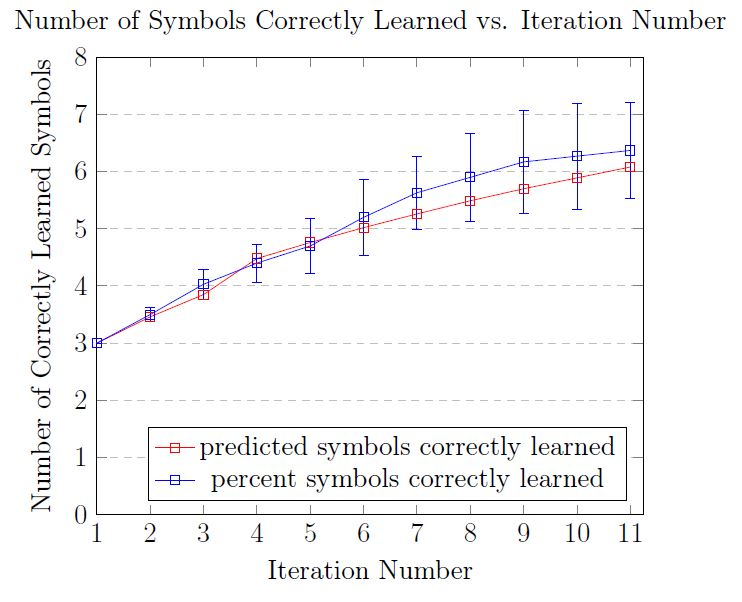
\includegraphics[width=\textwidth]{symbols_corr}
\caption{Number of learned symbols.}
\label{fig:symbols}
\end{subfigure}
\caption{The performance results of the simulation study.}
\end{figure}

\begin{figure}[h]
\centering
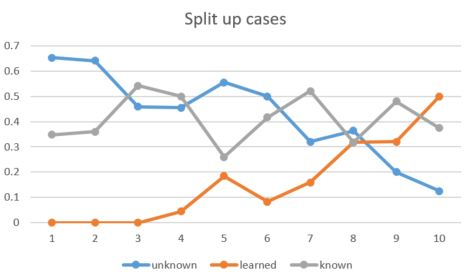
\includegraphics[width=0.7\columnwidth]{learning}
\caption{The percentage of symbols during the simulations.}
\label{fig:g_acc_split}
\end{figure}


%\begin{figure}[h]
%\centering
%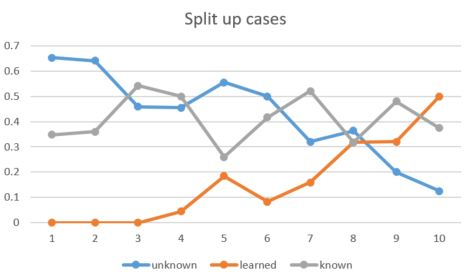
\includegraphics[width=8.5cm]{learning}
%\caption{this is split up (must replot well)}
%\label{fig:g_acc_split}
%\end{figure}


\subsection{Learned Symbols}
In order to better examine the learning behavior exhibited by the DCG-UPUP-Away model, the other performance metric considered is the number of correctly known symbols. Note that the symbols may be incorrectly learned by associating a phrase with the wrong sort of object due to the nature of unsupervised learning.
Initially, the turtlebot is trained with cubes, spheres, and cylinders, but the genrated environments may contain up to 5 additional object types (i.e., fire hydrants, drills, mailboxes, door handles, and traffic cones).
Whenever an unknown phrase is grounded to such an unknown object, the turtlebot learns the new symbol.
Thus, one may calculate the expected number of known symbols as a function of the iteration number using combinatorics to count how many unknown objects are present.
The recorded number of correctly learned symbols are plotted in Fig.~\ref{fig:symbols} in blue, as well as the expected number in red.
%\begin{figure}[h]
%\centering
%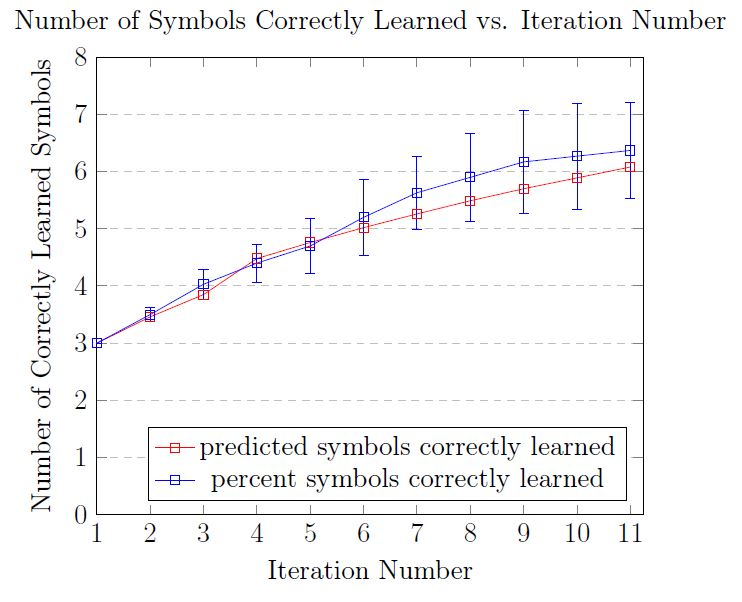
\includegraphics[width=8.5cm]{symbols_corr}
%\caption{this is how we show that we learn symbols. I will update this label (and caption) of this figure. also must use std error bars instead of variance}
%\label{fig:symbols}
%\end{figure}
%(Asking for advice: the x axis ranges from 1 to 11 because I can retrain after the 10th iteration and increase the mean number of symbols learned. It's a small increase, though, so I wouldn't be too upset cutting off the 11th iteration, though.)

As expected, the blue curve starts at $3$ (for the cube, sphere, and cylinder), and stochastically monotonically increases.
In $10\%$ of trials, all $8$ symbols were correctly learned. In other trials the DCG-UPUP-Away model incorrectly grounded unknown phrases (and therefore learned an incorrect symbol) or the 10 iterations collectively never referred to the five initially unknown objects, preventing the DCG-UPUP-Away model from ever learning the new symbol.
Furthermore, learning symbols correctly improves the grounding accuracy: for each additional correctly learned symbol, the turtlebot is over $4\%$ more likely to correctly ground a command. %(TODO generate p values via ANOVA.)

\subsection{Physical Demonstration}
In addition to the simulation studies, the DCG-UPUP-Away model was tested on an actual turtlebot in a laboratory setting.
The turtlebot was placed facing %a cylinder (known) and 
a cone (unknown).
In addition, a cube (known) and a crate (unknown) were located behind the turtlebot.
All objects were labeled with the AR-track tags \cite{olson2011}, which were used to generate the world model $\Upsilon$ from a kinect camera mounted on the turtlebot.

%I'd like to add a footnote saying that I have videos of these demos
Three natural language commands were used to demonstrate all capabilities of the DCG-UPUP-Away model.
%First, the turtlebot was given the command ``move towards the cube.''
%The turtlebot successfully drove to the cube, demonstrating a correct grounding to a known, perceived object.\\
First, the turtlebot was given the command ``move towards the cone.''
The turtlebot drove to the cone, demonstrating that it perceived the cone as unknown, recognized the phrase ``cone'' as unknown, and grounded the unknown phrase to the unknown object.
Thus, a command was correctly grounded to an unknown perceived object as illustrated in Fig.~\ref{fig:cone}.
Second, the turtlebot was given the command ``move towards the cube.''
The turtlebot rotated in place until the cube came in perception, and then approached the cube.
In other words, the command was first grounded to a known hypothesized object, and then it was grounded to a known perceived object once the cube was seen. 
Finally, the turtlebot was given the command ``move towards the crate.''
Once again, the turtlebot explored its surrounding by rotating at its current location and drove to the crate once it perceived it (as illustrated in Fig.~\ref{fig:crate}). %rotated in place, this time until it saw the crate, whereupon it drove to the crate.
The experimental results demonstrate two important behaviors: 1) the turtlebot must have learned what a cone was, otherwise the unknown phrase (``crate'') would have been grounded to the cone, and 2) the turtlebot grounded the command to an unknown hypothesized object until the crate was perceived. The interested reader is referred to the following link \footnote{\url{https://www.youtube.com/playlist?list=PL8sYMUToK9s6dAu3qMHHOef8FyhOnDK4E}} for the videos corresponding to these experiments.
%The execution of this last command, including images of the physical behavior of the turtlebot as well as the model used for grounding, is shown in Figure~\ref{fig:hardware_demo}.

%\begin{figure}[ht]
%\centering
%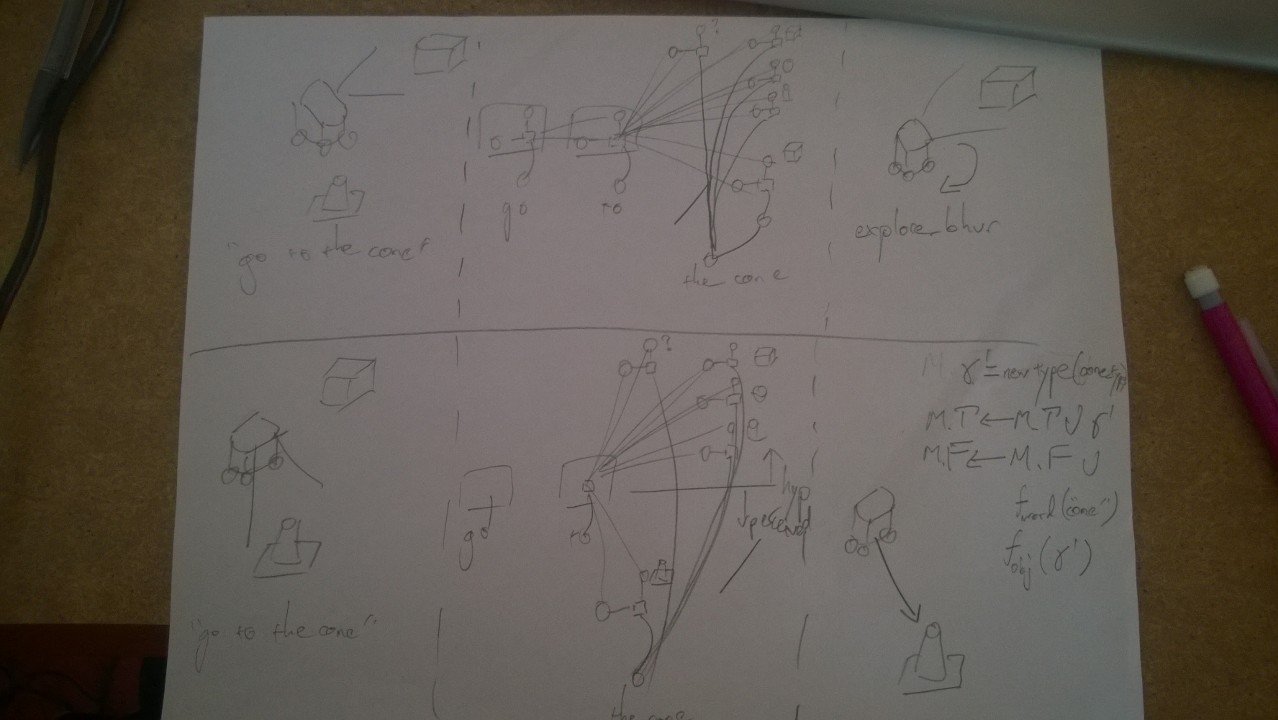
\includegraphics[width=8.5cm]{hardware_sketch}
%\caption{this is a sketch of the 6 subfigures that demonstrate hypothesized groundings on hardware and in the model, and shows how it learns. I'd like this to go across the top of the page.}
%\label{fig:hardware_demo}
%\end{figure}
%\begin{figure*}
%\begin{subfigure}[b]{0.31\textwidth}
%\centering
%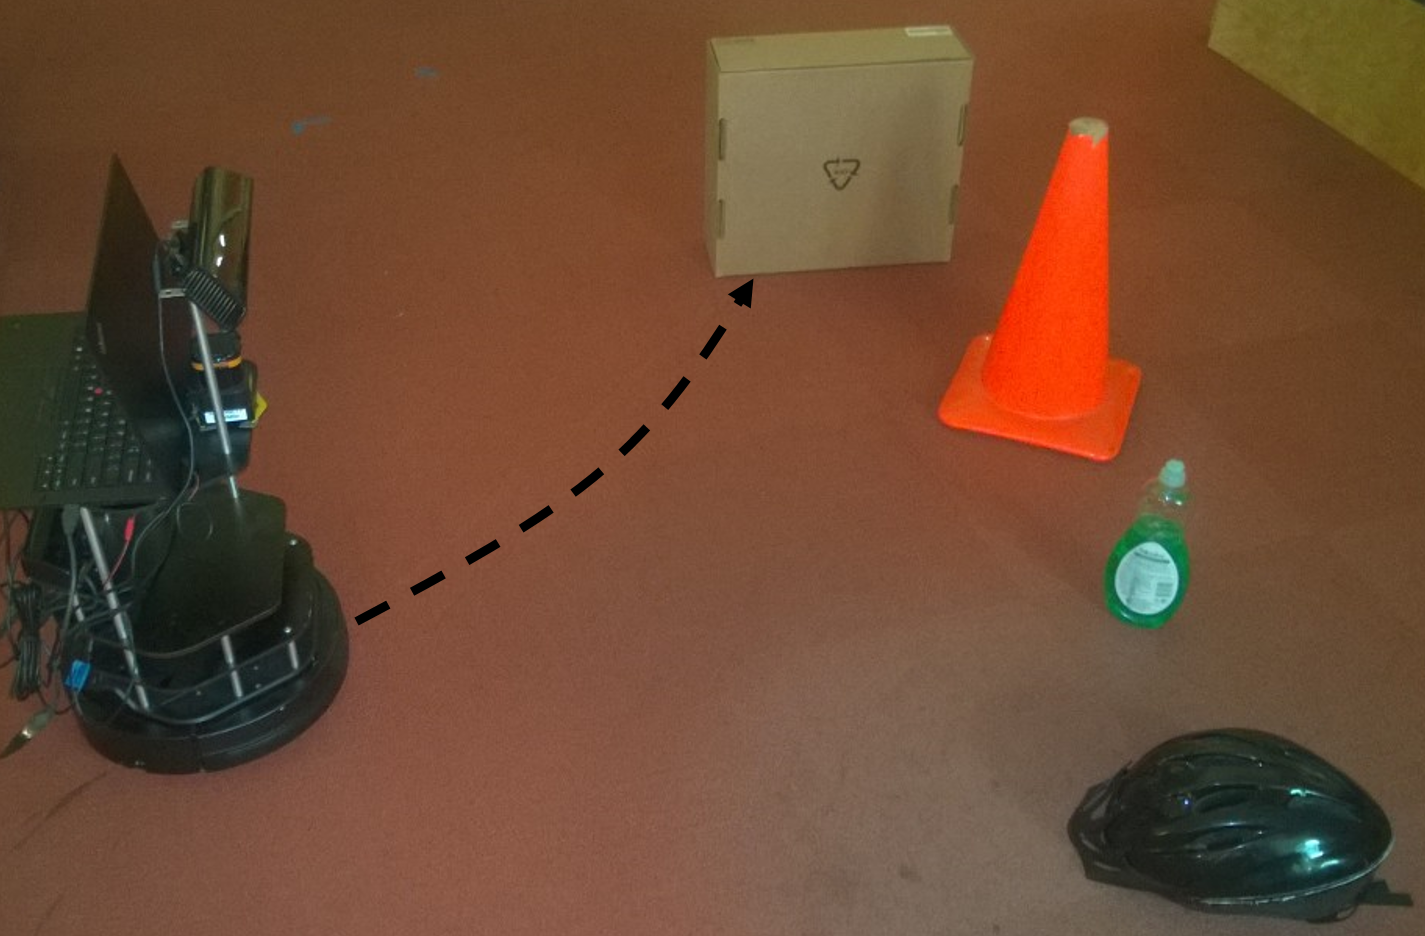
\includegraphics[width=\textwidth]{hardware1.png}
%\caption{The command ``move towards the box" is given, and the turtlebot approaches the box by grounding a known phrase to a known object.}
%\label{fig:g_acc}
%\end{subfigure}
%~
%\begin{subfigure}[b]{0.295\textwidth}
%\centering
%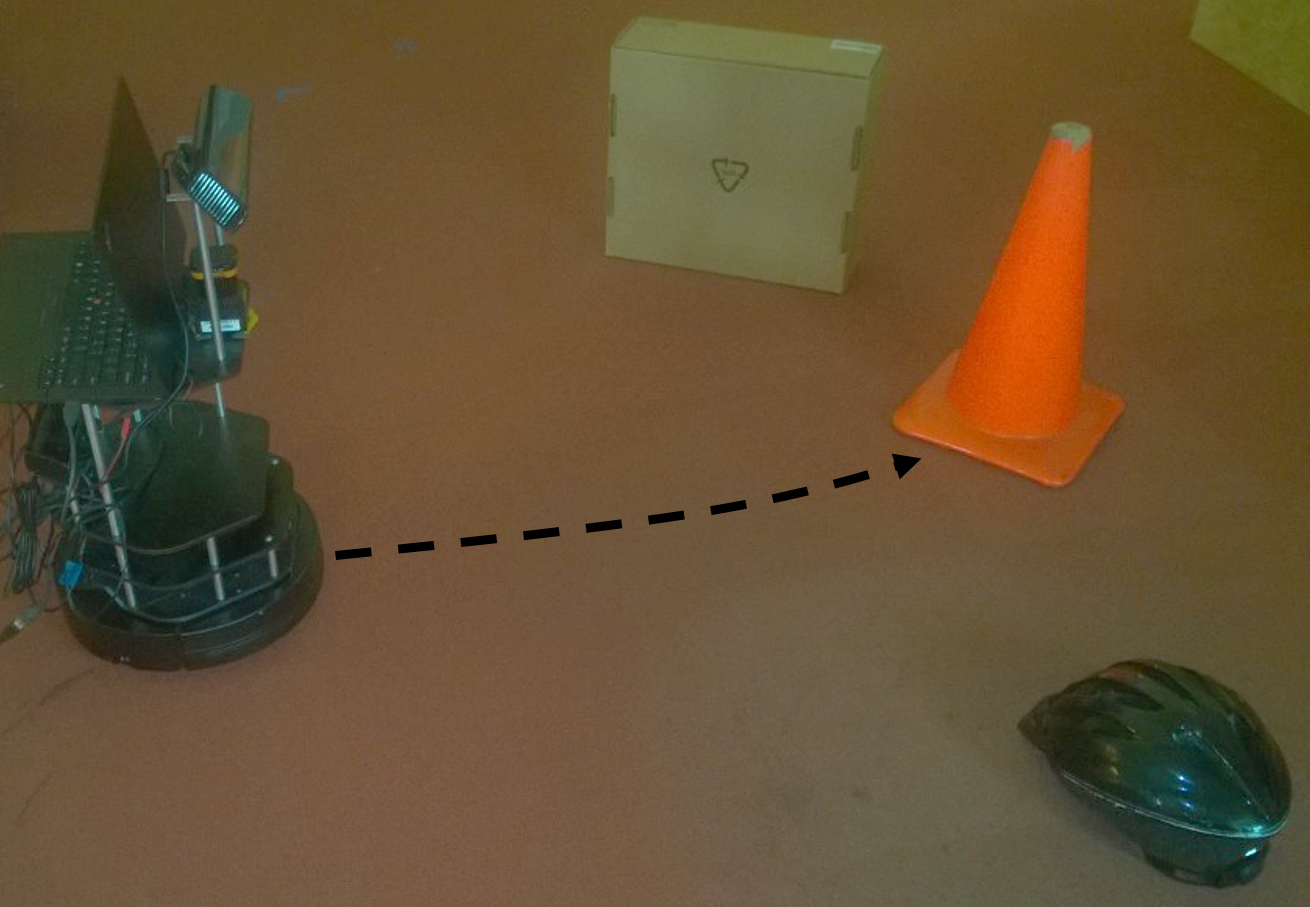
\includegraphics[width=\textwidth]{hardware2.png}
%\caption{The command ``move towards the cone" is given, and the turtlebot drives to the cone because unknown phrase ``cone" is grounded to the unknown object cone.}
%\label{fig:symbols}
%\end{subfigure}
%~
%\begin{subfigure}[b]{0.355\textwidth}
%\centering
%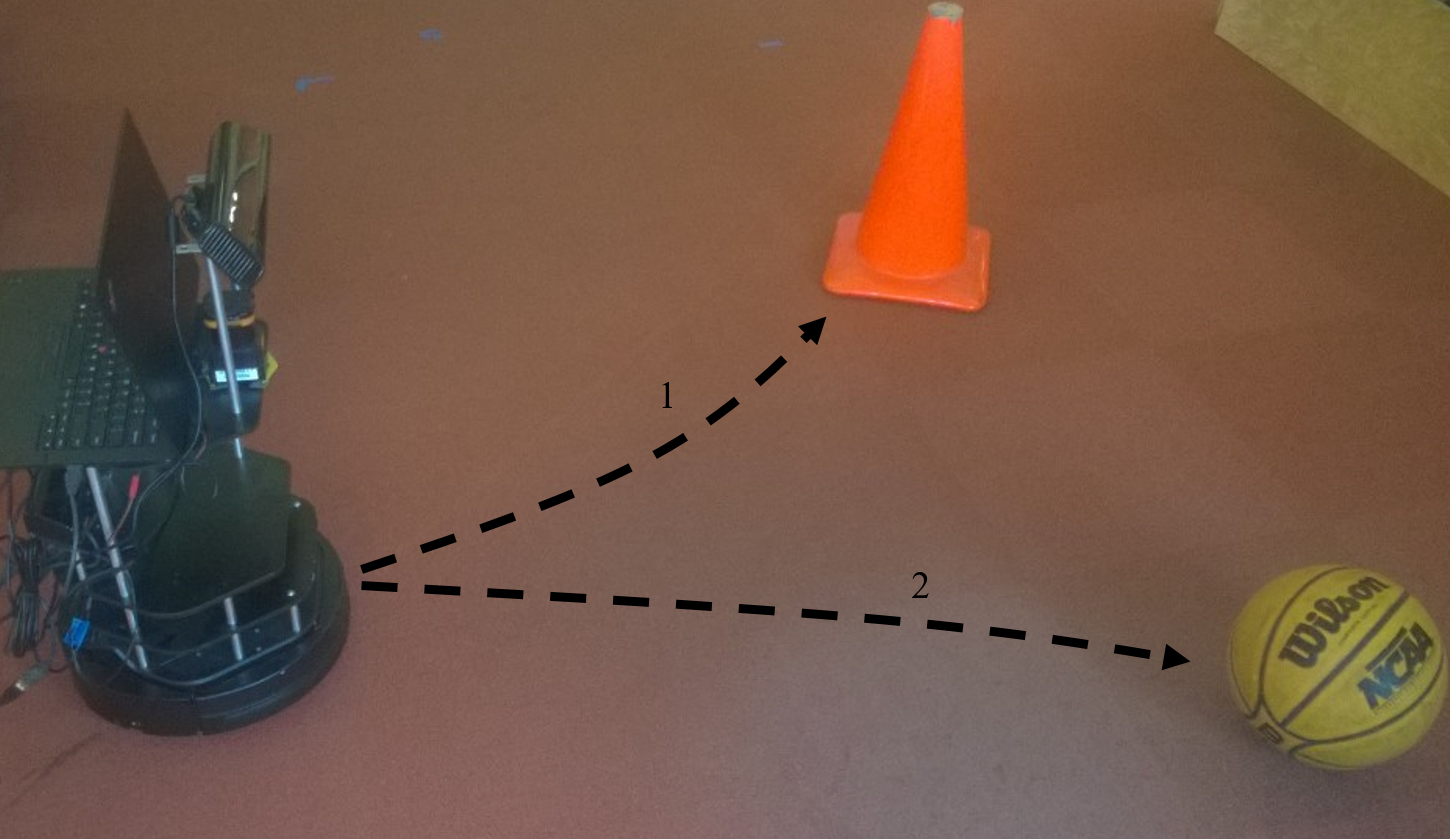
\includegraphics[width=\textwidth]{hardware3.png}
%\caption{The command ``move towards the cone" is given and the turtlebot follows path 1. The command ``move towards the ball" is given, and the turtlebot follows path 2.}
%\label{fig:g_acc_split}
%\end{subfigure}
%\caption{Some illustrations of iterative learning via the proposed model. (a) The turtlebot initially knows a box, a helmet, and a soap box, then (b) it learns what a cone is, and then (c) it learns what a ball is.}
%\end{figure*}


\begin{figure}
\begin{subfigure}[b]{0.305\columnwidth}
\centering
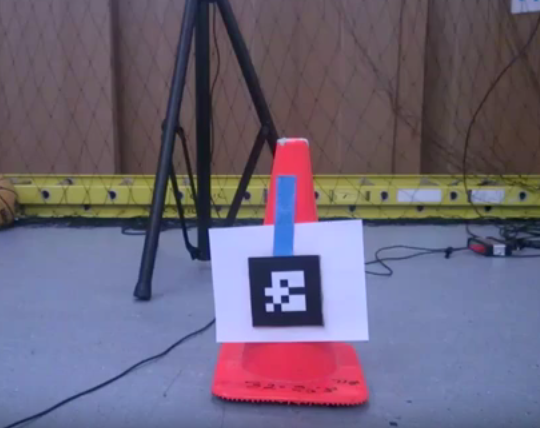
\includegraphics[width=\textwidth]{c1.png}
\caption{t= 0 sec.}
\label{fig:exp_new_1}
\end{subfigure}
~
\begin{subfigure}[b]{0.31\columnwidth}
\centering
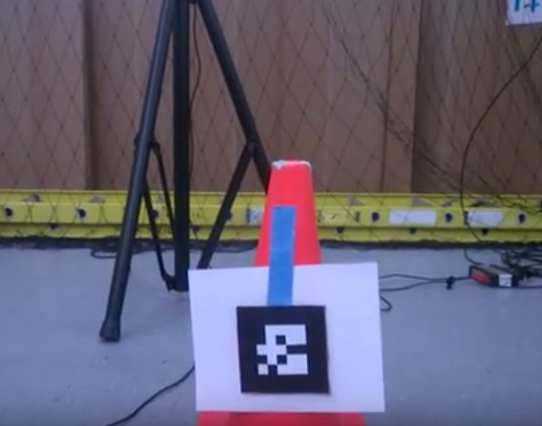
\includegraphics[width=\textwidth]{c2.png}
\caption{t= 45 sec.}
\label{fig:exp_new_2}
\end{subfigure}
~
\begin{subfigure}[b]{0.315\columnwidth}
\centering
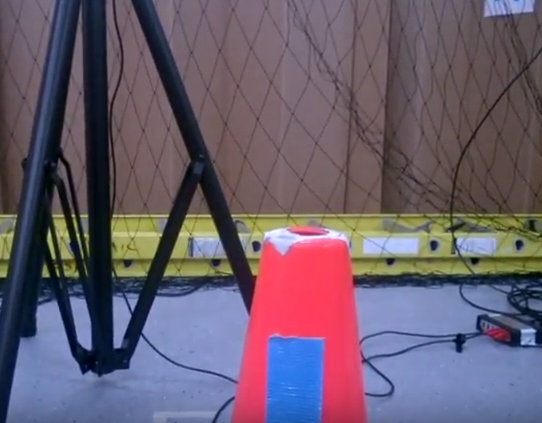
\includegraphics[width=\textwidth]{c3.png}
\caption{t= 50 sec.}
\label{fig:exp_new_3}
\end{subfigure}
\caption{An illustration of learning new symbol. The turtlebot initially does not know what a cone is, a command is given as ``move towards the cone". (a) Since there is an unknown object in its perceived world, it grounds the unknown phrase ``cone" to the unknown object, (b,c) it drives to the cone.}
\label{fig:cone}
\end{figure}

\begin{figure}[h!]
\begin{subfigure}[b]{0.45\columnwidth}
\centering
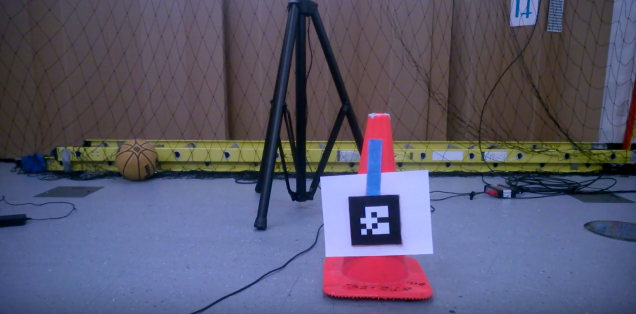
\includegraphics[width=\textwidth]{1.png}
\caption{t=0 sec.}
\label{fig:exp1}
\end{subfigure}
~
\begin{subfigure}[b]{0.45\columnwidth}
\centering
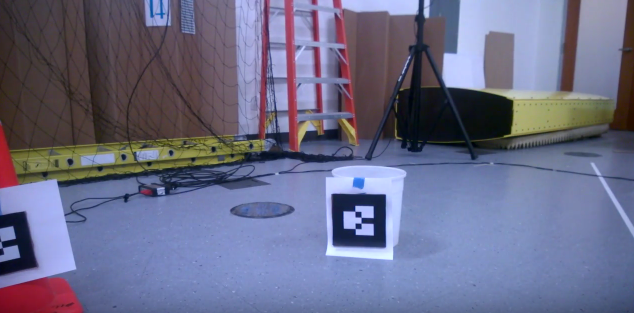
\includegraphics[width=\textwidth]{2.png}
\caption{t=25 sec.}
\label{fig:exp2}
\end{subfigure}
~
\begin{subfigure}[b]{0.45\columnwidth}
\centering
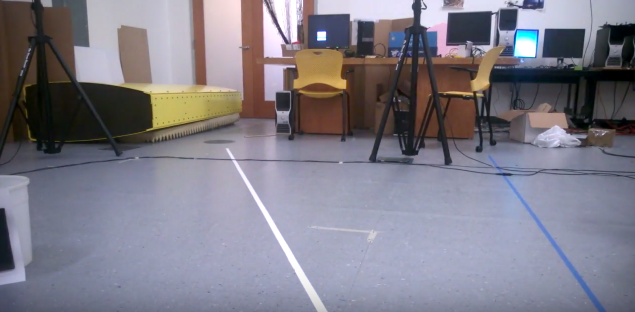
\includegraphics[width=\textwidth]{3.png}
\caption{t=50 sec.}
\label{fig:exp3}
\end{subfigure}
~
\begin{subfigure}[b]{0.45\columnwidth}
\centering
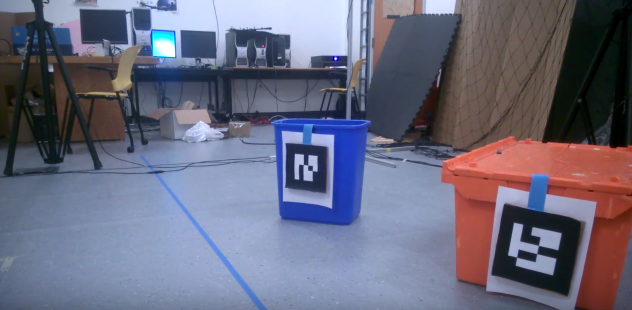
\includegraphics[width=\textwidth]{4.png}
\caption{t=70 sec.}
\label{fig:exp4}
\end{subfigure}
~
\begin{subfigure}[b]{0.45\columnwidth}
\centering
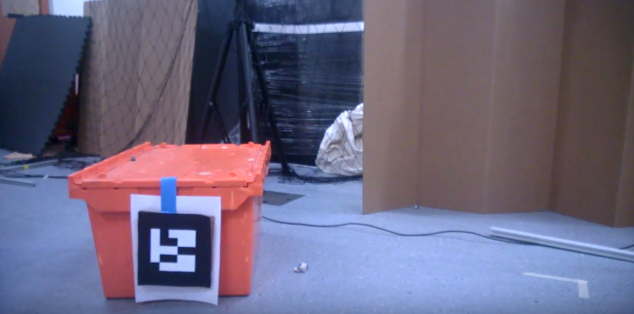
\includegraphics[width=\textwidth]{5.png}
\caption{t=95 sec.}
\label{fig:exp5}
\end{subfigure}
~~~~~~~
\begin{subfigure}[b]{0.45\columnwidth}
\centering
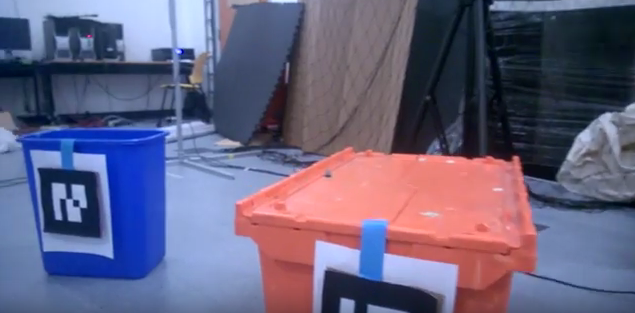
\includegraphics[width=\textwidth]{6.png}
\caption{t=120 sec. }
\label{fig:exp6}
\end{subfigure}
\caption{An illustration of grounding to a hypothetical object. The robot initially knows all objects in the world other than a crate. The turtlebot is given a command as ``move towards the crate". (a) First, it does not see an unknown object in its perceived world so it creates a hypothetical unknown object, (b,c,d) it explores the world by rotating at its current location until it perceives an unknown object, (e) It perceives an unknown object and grounds to it, (f) it drives to the crate.}
\label{fig:crate}
\end{figure}


\subsection{Limitations}
The previous sections demonstrated that the proposed model DCG-UPUP-Away results in the successful execution of various natural language commands. This section discusses the main limitations of the model.
%of the DCG-UPUP-Away model encountrduring  are equally important in characterizing the limits of its performance.\\
In particular, the most obvious limitation of the DCG-UPUP-Away model is the assumption of referring an unknown phrase to the first perceived unknown object. %that, in the absence of additional information, unknown phrases refer to the first perceived unknown object.
One strategy to relax this assumption has been explored in Section~\ref{sec:color} by associating language adjectives with object properties. However, a more sophisticated strategy is required for generalizable solutions.  %have been explored in Section (TODO color section), but so far only a relatively simple method has been used.\\
Moreover, the DCG-UPUP-Away model assumes a one-to-one correspondence between unknown phrases and unknown objects; thus it cannot, for example, learn synonyms by grounding unknown phrases to the known object types.
\section{Related Works}
\label{sec:related}
related work goes here
\section{Conclusion}
\label{sec:conclusion}
This paper addressed the problem of understanding natural language commands within a robot's symbolic world model. The main contribution of the paper was to propose a new probabilistic graphical model called DCG-UPUP-Away, which allows the explicit representation of 1) unknown phrases or objects, and 2) hypothetical objects that can be outside the field of view. Moreover, the proposed model has the capability to learn new symbols in an online fashion, so the learned phrases or objects become known when they are encountered again. The performance of the proposed model was evaluated via simulations and real experiments, where a turtlebot was used and various natural language commands were given. The results indicated that the DCG-UPUP-Away model can ground correct objects approximately $80\%$ of the time. Some potential future directions can be extending the model to reason about multiple unknown (hypothetical) objects or understanding the synonyms of known objects.
\section{Future Work}
\label{sec:future}
future work goes here
\section*{Acknowledgments}
This work was supported in part by the Robotics Consortium of the U.S Army Research Laboratory under the Collaborative Technology Alliance Program.\\

\input{appendix}
\printbibliography

\end{document}